\documentclass{moncours}
\usepackage{float}
\usepackage{amssymb}
\makeindex




\begin{document}

\newcounter{tmp} % pour couper les boîtes énoncés au milieu d'un enumerate

\renewcommand{\labelitemi}{\textbullet}
\renewcommand{\labelitemii}{$\circ$} 

\frontmatter

\titlePage[./images/couvertureFlo4e_v11]{Informatique 4\up{e}}{Fiches MITIC}{Institut Florimont}{Petit-Lancy (Suisse)\\ \textcopyright\ Tout droit réservé. Crédit photographie couverture : Institut Florimont. Illustration des premières pages de chapitre issue de \emph{Codex Leicester} de Leonardo da Vinci (domaine public).  \\ 2\up{ème} édition v2.0\\juin 2021} 

% Commentaires ou erreurs à signaler à \texttt{flo-mitic@florimont.ch}

% TOC
\pagestyle{empty} % No headers

\tableofcontents % Print the table of contents itself
\cleardoublepage % Forces the first chapter to start on an odd page so it's on the right
\pagestyle{fancy} % Print headers again

\cleardoublepage % on force une page impaire
\vspace*{1cm}

\section*{Calendrier des différentes activités (4\up{e})}\index{Calendrier des activités}  

\vfill

\begingroup % permet de bloquer le arraystretch à ce groupe seulement
\renewcommand{\arraystretch}{1.2}
\begin{center}
\begin{tabular}{|l|l|c|l|l|}
\hline
\multirow{2}{*}{\textbf{Nom de la fiche}} & \multirow{2}{*}{\textbf{Matière}} & \multirow{2}{*}{\textbf{Page}} & \textbf{Date de} & \textbf{Nom du} \\
 &  &  & \textbf{réalisation} & \textbf{professeur} \\ \hline
%\rowcolor[gray]{0.8}\multicolumn{5}{|l|}{Rentrée scolaire} \\ \hline 
%\emph{La plateforme Flore} & (Titulaire) & \pageref{plateformeFlore} & & \phantom{xxxxxxxxxxxxxxxx}  \\ \hline
%
% avant les vacances d'octobre
%
\rowcolor[gray]{0.8}\multicolumn{5}{|l|}{Avant les vacances d'octobre} \\ \hline
\emph{Tableur : séance 1} & Mathématiques & \pageref{ficheTableur4e1} & & \\ \hline
\emph{Texte : séance 1} & Anglais & \pageref{ficheTexte4e1} & & \\ \hline

\multicolumn{5}{l}{} \\ \hline % saut ligne

%
% avant les vacances de Noël
%
\rowcolor[gray]{0.8}\multicolumn{5}{|l|}{Avant les vacances de Noël} \\ \hline
\emph{Texte : séance 2} & Français & \pageref{ficheTexte4e3} & & \\ \hline
\emph{Scratch : séance 1} & Mathématiques & \pageref{ficheScratch4e1} & & \\ \hline

\multicolumn{5}{l}{} \\ \hline % saut ligne

%
% avant les vacances de février
%
\rowcolor[gray]{0.8}\multicolumn{5}{|l|}{Avant les vacances de février} \\ \hline
\emph{Image : séance 1} & SVT & \pageref{ficheImage4e2} & & \\ \hline


\multicolumn{5}{l}{} \\ \hline % saut ligne

%
% avant les vacances de printemps
%
\rowcolor[gray]{0.8}\multicolumn{5}{|l|}{Avant les vacances de printemps} \\ \hline
\emph{Tableur : séance 2} & Sciences physiques & \pageref{ficheTableur4e2} & & \\ \hline
\emph{Texte : séance 3} & Mathématiques & \pageref{ficheTexte4e2} & & \\ \hline
\emph{Scratch : séance 2} & Mathématiques & \pageref{ficheScratch4e2} & & \\ \hline
%\emph{Son : séance 2} & Anglais & \pageref{ficheSon4e2} & & \\ \hline

\multicolumn{5}{l}{} \\ \hline % saut ligne


%
% avant les vacances d'été
%
\rowcolor[gray]{0.8}\multicolumn{5}{|l|}{Avant les vacances d'été} \\ \hline
\emph{Image : séance 2} & Français & \pageref{ficheImage4e1} & & \\ \hline
\emph{Scratch : séance 3} & Mathématiques & \pageref{ficheScratch4e3} & & \\ \hline

\multicolumn{5}{l}{} \\ \hline % saut ligne


%
% avant la fin du semestre de cours
%
\rowcolor[gray]{0.8}\multicolumn{5}{|l|}{Avant la fin du semestre de cours (pour les cours au semestre)} \\
 \hline %\emph{Tableur : séance 3} & Géographie & \pageref{ficheTableur4e3} & & \\ \hline
\emph{Image : séance 3} & Arts visuels & \pageref{ficheImage4e3} & & \\ \hline
%\emph{Son : séance 1} & Musique & \pageref{ficheSon4e1} & & \\ \hline
\end{tabular}
\end{center}
\endgroup

\vfill

\cleardoublepage % on force une page impaire pour le clavier
\section*{Les touches spéciales du clavier}\index{Clavier}\index{Touches spéciales}

\vfill

\begin{center}
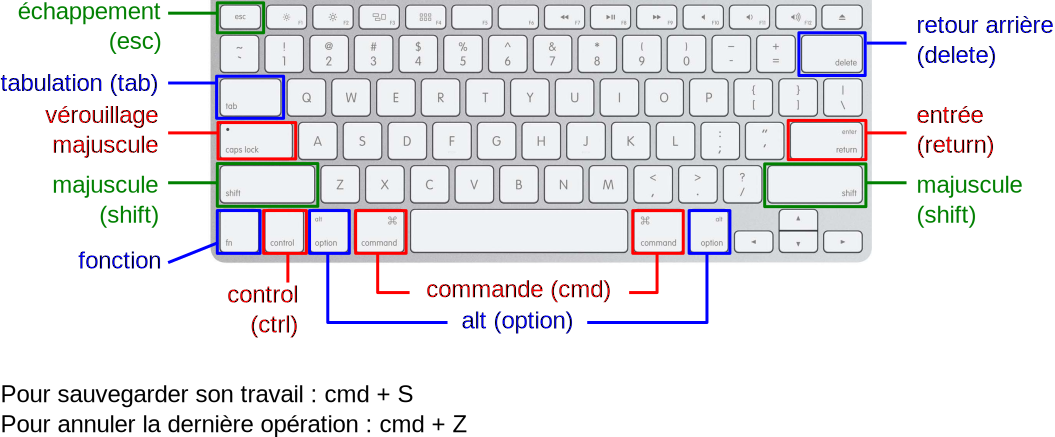
\includegraphics[angle=90,width=.6\textwidth]{./images/generales/clavierTouches}
\end{center}

\vfill

\cleardoublepage % on force une page impaire pour la philosophie du document
\chapter*{Philosophie du document}


\prof{\textbf{ceci est la version professeur du document.} L'icône du professeur est suivie par des informations complémentaires qui n'apparaissent pas dans la version élève.}  

Vous avez entre les mains le deuxième tome d'une série de trois fascicules qui accompagneront les élèves des classes de 6\up{e}, 5\up{e}, 4\up{e} ET 3\up{e} jusqu'au moment où ils recevront un ordinateur qu'ils seront en mesure d'exploiter au mieux pour leur travail.

\vspace{18pt}

Ce document se présente sous la forme d'un livret qui rassemble des fiches MITIC\footnote{MITIC : Médias, Images et Technologies de l'Information et de la Communication.} permettant aux élèves d'apprendre à utiliser les logiciels et espaces numériques mis à leur disposition. Pour l'année de 5\up{e}, sont traités les logiciels \emph{Microsoft Word} (traitement de texte), \emph{Microsoft Excel} (tableur grapheur), \emph{Gimp} (retouche d'image), \emph{Audacity} (traitement des fichiers son) et \emph{Scratch} (programmation). Au début de chaque chapitre un lien permettant de télécharger le logiciel est fourni.

\vspace{18pt}


Chaque fiche est conçue pour être exploitée à plusieurs occasions et dans des matières différentes, à chaque fois lors d'une séance de 45 minutes. La fiche sur le tableur, par exemple, est découverte en physique-chimie (\emph{Séance 1}), exploitée à nouveau en mathématiques (\emph{Séance 2}) puis en histoire-géographie (\emph{Séance 3}) selon un calendrier proposé en début de fiche. Nous avons à chaque fois essayé de faire coïncider les notions abordées dans la fiche avec le programme de la matière concernée.

\vspace{18pt}

Professeurs, c'est à vous que revient la tâche délicate d'inclure le contenu de ces fiches dans votre progression. À vous de le faire vivre : arriver en salle informatique et demander aux élèves de remettre en forme un texte de Molière ne présente que peu d'intérêt pédagogique. Donnez du sens à ces fiches et profitez-en pour diversifier votre enseignement. N'hésitez pas à exploiter dans vos cours les techniques présentées dans ce fascicule afin que les élèves utilisent plusieurs fois leurs nouvelles compétences et, par là-même, les pérennisent.

%\vspace{18pt}

%Ces fiches MITIC sont appelées à évoluer. N'hésitez pas à nous transmettre vos suggestions et nous signaler toute erreur relevée par courriel à l'adresse \texttt{flo-mitic@florimont.ch}.

\vspace{18pt}

Merci d'avance à tous pour votre implication.

\vspace{18pt}

L'équipe de rédaction.

\vspace{2cm}

% \emph{Remarque : il existe une version professeur de ce document, contenant des informations complémentaires, disponible sur l'ENT de l'école.}

  


% Début des chapitres
%\setcounter{page}{1} % si on veut forcer la page 1 au début du premier chapitre
\mainmatter
%
  
% ETAT DES SOURCES
% texte03 OK
% scratch03 OK
% images03 OK
% son02 projet

% ETAT DES IMAGES
% texte03 OK
% tableur03 OK
% images03 OK
% scratch03 OK 

\chapterImage{./images/chapitreVinci4e}
\documentclass{article}
\usepackage[utf8]{inputenc}
\usepackage{graphicx}
\usepackage{wrapfig}
\usepackage{caption}


\begin{document}

\section{Connexion à Office 365 et Teams}

Nikolai

Possibilité de télécharger l'application

\section{Apparence de la page d'accueil}

La page d'accueil de Teams se présente sous forme d'une liste de classes 

\begin{figure}[h]
\includegraphics[width=5cm]{accueil_liste.png}
\centering
\end{figure}

ou sous forme d'une grille de classes \newpage

\begin{figure}[h]
\includegraphics[width=10cm]{accueil_grille.png}
\centering
\end{figure}

Pour passer d'une forme à l'autre, il faut cliquer sur le sigle \includegraphics[width=0.7cm]{bouton_parametres.png}, choisir \textit{Changer d'affichage} dans le menu déroulant, comme dans l'exemple illustré ci-dessous :

\begin{figure}[h]
\includegraphics[width=10cm]{changement_liste.png}
\centering
\end{figure}

il faut ensuite sélectionner le type d'affichage souhaité entre \textit{Grille} et \textit{Liste}
\newpage

\begin{figure}[h]
\includegraphics[width=12cm]{choix_parametre.png}
\centering
\end{figure}

 Pour entrer maintenant dans votre classe, dans la matière de votre choix, il suffit de cliquer sur l'icône correspondante

\begin{figure}[h]
\includegraphics[width=12cm]{entree_classe.png}
\centering
\end{figure}

\newpage

\section{Utilisation de la messagerie}

La messagerie instantanée proposée par Teams doit permettre aux élèves et aux enseignants de communiquer en dehors de l'école dans un cadre qui reste strictement scolaire. Ainsi les messages personnels n'ont aucune raison d'être sur Teams. Il n'est par ailleurs pas possible pour un élève de supprimer un message envoyé. Seul le modérateur de la classe peut procéder à une telle suppression. 

Par ailleurs, toute forme d'insulte, de jugement personnel ou de critique envers un membre de la classe est à proscrire.



\section{Consulter et télécharger un document}

Nikolai

\section{Déposer un devoir}

Pour consulter les devoirs déposés par votre enseignant, il faut choisir \textit{2 de plus} dans la barre de menus du haut de page, puis sélectionner \textit{Devoirs}.

\begin{figure}[h]
\includegraphics[width=10cm]{devoir1.png}
\centering
\end{figure}

La page qui s'affiche maintenant fait le bilan de ce qui a déjà été fait et des devoirs proposés par votre enseignant. En cliquant sur \textit{Rédaction} vous pourrez accéder au devoir.

\begin{figure}[h]
\includegraphics[width=10cm]{devoir2.png}
\centering
\end{figure}

\newpage
 Vous obtenez alors l'écran suivant

\begin{figure}[h]
\includegraphics[width=12cm]{devoir3.png}
\centering
\end{figure}

Il est maintenant possible de consulter le sujet sous forme de pièce jointe en sélectionnant ...

\section{Accéder à mon carnet}

\section{Rejoindre une visio-conférence}


\end{document}
\chapter{Tableur}  

Un tableur est un logiciel qui permet de faire des calculs à partir de tableaux contenant des nombres (les \emph{données}). Un tableur permet également de représenter ces données sous forme de graphiques qui en facilitent généralement la lecture.

\phantom{rien}

{\footnotesize
\begin{itemize}
\item Logiciel : \emph{Microsoft Excel}
\item Matières concernées : mathématiques, sciences physiques et géographie.
\item Compétences : 
        \begin{itemize}
        \item importer un fichier au format \texttt{CSV} ;
        \item référence variable et référence fixe ;
        \item trier des données ;
	\item fixer une ligne ou une colonne à l'affichage ;
	\item utiliser une condition pour définir le contenu d'une cellule ;
	\item naviguer dans une grande feuille de calcul.
        \end{itemize}
\item Cette fiche est à réaliser :
        \begin{itemize}
        \item avant les vacances d'octobre en mathématiques (séance 1) ;
        \item avant les vacances de printemps en sciences physiques (séance 2) ;
        \item avant la fin du semestre de cours en géographie (séance 3). 
        \end{itemize}
\end{itemize}
}% fin du footnotesize





\section*{Les années précédentes, vous avez appris...}

Les compétences listées ci-dessous ont été vues en classes de 6\up{e} et de 5\up{e}. Vous en aurez à nouveau besoin pour les activités de cette année. Si nécessaire, reportez-vous aux \emph{Fiches MITIC} des années précédentes pour revoir comment :  

\begin{itemize}
\item insérer une formule dans une cellule (6\up{e}) ;
\item utiliser la recopie incrémentale (6\up{e}) ;
\item tracer un graphique (nuage de points) (6\up{e}) ;
\item exporter la feuille et le graphique obtenus (6\up{e}) ;
\item définir le format d'une cellule (5\up{e}) ;
\item insérer une courbe de tendance dans un graphique (5\up{e}) ;
\item mettre en page une feuille de calcul (5\up{e}) ;
\item réaliser un diagramme circulaire (5\up{e}) ;
\item exporter un graphique, un tableau (5\up{e}).
\end{itemize}





%
%
%  S  É  A  N  C  E     I
%
%

\newpage

\section{Séance 1 : Moyennes avec coefficients (maths)}\label{ficheTableur4e1}

\subsection{Pour bien démarrer...}

Dès que vous avez ouvert un nouveau document dans \emph{Excel}, sauvegardez-le au format Nom-date.xlsx : dans le menu \texttt{Fichier}, choisir \texttt{Enregistrer}. Pendant que vous travaillez, pensez à sauvegarder régulièrement votre travail (raccourci clavier \texttt{Cmd + s}).   

\uneimageici{./images/generales/clavierCmdS}{.4\textwidth}

%\vspace{10pt}

\subsection{L'activité demandée}

\vspace{10pt}


\boiteEnonceLarge{%
Le but de cette séance est de faire le calcul de la moyenne des élèves de 4\up{e} d'un établissement et de donner des informations par classe sur les résultats.

\vspace{6pt}

À partir du fichier \texttt{ListeEleves\&Notes.csv} fourni par votre enseignant sur \emph{Teams}, il faut :
\begin{itemize}
\item figer les cellules pour que la première ligne soit toujours apparente;
\item trier les données pour trouver le meilleur élève de l'établissement, toutes classes confondues. Copier et coller son nom et sa moyenne dans les cellules \texttt{N3} et \texttt{O3};
\item calculer dans la cellule \texttt{I3} la moyenne de la première élève de la liste en tenant compte des coefficients qui se trouvent dans les cellules \texttt{E2} à \texttt{H2}.
\item tirer (recopie incrémentale) la formule trouvée pour obtenir la moyenne de tous les élèves (attention aux références variables);
\item dans la cellule \texttt{J3}, entrer la formule qui indique si l'élève est promu(e) ou redouble (condition sur la moyenne annuelle qui vient d'être calculée dans la colonne \texttt{I} puis tirer cette formule pour tous les élèves) ;
\item dans la cellule \texttt{K3}, écrire le texte «\,Nombre d'élèves promus :\,» et dans la cellule \texttt{L3}, entrer la formule qui calcule ce nombre automatiquement;
\end{itemize}
}

\boiteEnonceLarge{
\begin{itemize}
\item entrer le texte «\,nb. de redoublants :\,» dans la cellule \texttt{K4} puis tirer la formule entrée en \texttt{L3} dans la cellule \texttt{L4} (attention aux références variables) puis la modifier pour obtenir le nombre de redoublants;
\item trier les données par classe puis par moyenne pour donner le meilleur élève de chacune des classes (copier et coller le nom de l'élève et sa moyenne générale dans les cellules \texttt{N5} à \texttt{O12};
\item trier les élèves par classe puis calculer la moyenne de chacune des classes en utilisant la fonction \texttt{SOMME} pour calculer la somme des notes et \texttt{NB.SI} pour calculer le nombre d'élèves de la classe.
\end{itemize}
\vspace{10pt}
Une fois la mise en forme terminée, enregistrer le document au format \texttt{.xlsx} en le nommant à partir de votre nom : \texttt{Nom-date.ods} puis rendre ce fichier sur \emph{Teams} à l'endroit indiqué par votre enseignant (si nécessaire, se reporter à la fiche méthode \emph{Remettre un devoir sur Teams}).
} % fin énoncé

\textbf{Pour obtenir de l'aide, rendez-vous à la page \pageref{AideTableur03}}

\section{Pour aller plus loin...}
Vous avez appris à utiliser trois fonctions du tableur : \texttt{SI}, \texttt{NB.SI} et \texttt{SOMME}. Mais il en existe beaucoup d'autres qui permettent d'automatiser de très nombreux calculs. Pour les découvrir et découvrir comment les utiliser, vous pouvez utiliser le \texttt{Concepteur de formules} :
\uneimageici{./images/tableur03/IconeFonction_Excel_crop}{\textwidth}

\begin{itemize}
\item pour une meilleure lisibilité, utiliser la fonction \texttt{ARRONDI.AU.MULTIPLE} et afficher les moyennes arrondies au centième;
\item calculer la moyenne d'une classe en triant les données par \texttt{classe} puis en utilisant la fonction \texttt{MOYENNE} (déjà vue en 6\up{e}) ; tirer la formule trouvée dans les 7 cellules adjacentes pour obtenir les moyennes des 7 autres classes (attention aux références variables);
\item calculer la moyenne par classe sans avoir besoin de trier les données en utilisant les fonctions \texttt{NB.SI} et \texttt{SOMME.SI}.
\end{itemize}

\vfill

%\cadre{Pensez à sauver régulièrement votre travail en appuyant sur \texttt{Cmd + S} ou à partir du menu \texttt{Fichier} en choisissant \texttt{Enregistrer}.

%\uneimageici{./images/generales/clavierCmdS}{.5\textwidth}
%}






%
%
%  S  É  A  N  C  E     II
%
%


\pagebreak

\section{Séance 2 : Traitement de données (Sc. physiques)}\label{ficheTableur4e2}

\subsection{Pour bien démarrer...}

Dès que vous avez ouvert un nouveau document dans \emph{Excel}, sauvegardez-le au format Nom-date.xlsx : dans le menu \texttt{Fichier}, choisir \texttt{Enregistrer}. Pendant que vous travaillez, pensez à sauvegarder régulièrement votre travail (raccourci clavier \texttt{Cmd + s}).   

\uneimageici{./images/generales/clavierCmdS}{.4\textwidth}

%\vspace{10pt}

\subsection{L'activité demandée}

\vspace{10pt}


\boiteEnonceLarge{%
Le but de cette séance est de réaliser le traitement de données brutes fournies par la centrale d'acquisition ExAO de l'école. Les données collectées par ExAO sont exportées au format \texttt{CSV} (dans le logiciel \emph{Latis}, menu \texttt{Fichier}, choisir \texttt{Exportation} puis choisir le format de fichier \texttt{CSV}). 

\vspace{6pt}

Le fichier \texttt{CSV} est alors importé dans \emph{Excel} où les données sont traitées selon les consignes données par votre enseignant.

\vspace{6pt}

Une fois votre travail terminé, exporter votre graphique au format PNG en le nommant à partir de votre nom : \texttt{Nom-date.png} puis rendre ce fichier sur \emph{Teams} à l'endroit indiqué par votre enseignant (si nécessaire, se reporter à la fiche méthode \emph{Remettre un devoir sur Teams}).
}% fin énoncé



%\cadre{Pensez à sauver régulièrement votre travail en appuyant sur \texttt{Cmd + S} ou à partir du menu \texttt{Fichier} en choisissant \texttt{Enregistrer}.

%\uneimageici{./images/generales/clavierCmdS}{.5\textwidth}
%}

\textbf{Pour obtenir de l'aide, rendez-vous à la page \pageref{AideTableur03}}
\vfill

%
%
%  S  É  A  N  C  E     III
%
%



%\pagebreak

%\section{Séance 3 : Ressources en eau (géographie)}\label{ficheTableur4e3}

%\boiteEnonceLarge{%
%Le but de cette séance est de retrouver et calculer des données dans un fichier au format \texttt{CSV} pour étudier les ressources en eau douce sur la planète. Pour cela :
%\begin{itemize}
%\item importer un fichier au format \texttt{CSV} dans \emph{LibreOffice Calc} ;
%\item utiliser le tri de données pour faire apparaître le classement des pays en fonction de différents critères ;
%\item déterminer à quel groupe les pays appartiennent en fonction de leurs ressources en eau en utilisant la fonction \texttt{SI};
%\item calculer le nombre de pays appartenant à différents groupes en fonction de leurs ressources en eau, en utilisant la fonction \texttt{NB.SI};
%\item insérer un diagramme circulaire représentant les ressources en eau des différents groupes.
%\end{itemize}
%Une fois la mise en forme terminée, exporter le document au format ODS en le nommant à partir de votre nom : \texttt{Nom-Prénom-date.ods} puis rendre ce fichier sur la plateforme \emph{Moodle} à l'endroit indiqué par votre enseignant (si nécessaire, se reporter à la fiche méthode \emph{Remettre un devoir sur Moodle}, section \vref{MoodleRendreDevoir}).
%}% fin énoncé


%Récupérer sur \emph{Moodle} le fichier nommé \texttt{Geographie\_Eau\_Tableau.csv}, l'ouvrir avec \emph{LibreOffice Calc} et l'enregistrer au format ODS (\texttt{Nom-Prénom-date.ods}). Dans ce fichier, au départ, les pays sont classés par ordre alphabétique.

%\subsection{Ressources en eau des différents pays}

%\subsubsection{Ressources en eau par habitants}

%Pour calculer les ressources en eau (nombre de m\up{3} par habitant\footnote{Un mètre-cube (m\up{3}) correspond à 1000\,litres}), entrer la formule permettant de faire le calcul pour le premier pays dans la cellule \texttt{G2} puis faire une recopie incrémentale de cette formule pour tous les pays.

%\emph{Remarque :} la colonne des ressources en eau donne des valeurs en milliards de m\up{3}. Pour calculer les ressources en eau par habitant en \texttt{m\up{3} par habitant}, il faut multiplier le résultat par $10\up{9}$. Pour cela, on entre dans la cellule la formule suivante : \texttt{=(E2/F2)*10}\texttt{\^}\texttt{9}.

%Trier ensuite les pays en fonction de la ressource en eau par habitant. Indiquer les 5 pays les plus «\,riches\,» en eau et les 5 pays les moins bien dotés par rapport à leur population en faisant un copier/coller de ces pays dans les cellules \texttt{K2} à \texttt{K6} et \texttt{K8} à \texttt{K12}.

%\subsubsection{Ressources en eau par km\up{2}}

%Entrer la formule permettant de faire le calcul des ressources en eau (en m\up{3}) par km\up{2} dans la colonne \texttt{H}.

%Indiquer les 5 pays les plus «\,riches\,» et les 5 pays les moins bien dotés par rapport à leur superficie en faisant un copier/coller de ces pays dans les cellules \texttt{M2} à \texttt{M6} et \texttt{M8} à \texttt{M12}.


%\subsubsection{Ressources en eau totales}

%Trier les données du fichier pour identifier les 9 pays qui ont le plus de réserve en eau. Dans une cellule de votre choix, calculer la ressource en eau totale pour tous les pays et dans une autre cellule, la ressource en eau de ces 9 pays. Dans une troisième cellule, calculer le pourcentage d'eau possédée par ces pays (que vous pourrez comparer avec la valeur annoncée dans le document utilisé dans la partie \emph{Pour aller plus loin...}). Attention, pour les calculs des pourcentages, il faudra utiliser une référence fixe (se reporter au \S\ \vref{Calc3reference}).

%\subsection{Ressources en eau, classement des pays en trois groupes}

%Réaliser, dans la colonne \texttt{I}, les classement des pays en fonction du critère suivant : les pays qui disposent de moins de $\numprint{1000}$ m\up{3} d'eau par habitant et par an sont classés dans le groupe des pays \texttt{pauvres en eau}. Les pays ayant entre $\numprint{1000}$ et $\numprint{8000}$ m\up{3} sont classés dans les pays \texttt{Moyennement dotés}. Enfin, les pays ayant plus de $\numprint{8000}$ m\up{3} d'eau par habitant et par an sont classés dans le groupe des pays $\texttt{Riches en eau}$.
%\begin{enumerate}
%\item Dans la cellule \texttt{I2}, entrer la condition. Comme il y a trois cas possibles, les trois paramètres de la fonction \texttt{SI} sont les suivants : 
%  \begin{itemize}
%    \item le premier paramètre est la première condition : \texttt{G2 < $\numprint{1000}$} ;
%    \item le deuxième paramètre est la valeur si la première condition est vraie : \texttt{"Pauvre en eau"};
%    \item le dernier paramètre est la valeur si la première condition est fausse. Ce paramètre va à nouveau être une condition \texttt{SI} qui contient trois paramètres :
%	\begin{itemize}
%	  \item le premier paramètre est la deuxième condition : \texttt{G2 < $\numprint{8000}$} ;
%	  \item le deuxième paramètre est la valeur si la deuxième condition est vraie : \texttt{"Moyennement doté"};
%	  \item le troisième paramètre est la valeur si la deuxième condition est fausse : \texttt{"Riche en eau"}.
%	\end{itemize}  
%  \end{itemize}
%\item Une fois la formule de la cellule entrée correctement, la tirer vers le bas pour avoir cette formule pour tous les pays.
%\item Dans la cellule \texttt{I174}, calculer le nombre de pays \emph{«\,Pauvre en eau\,»} en utilisant la fonction \texttt{NB.SI}. Le premier paramètre à entrer est la liste des cellules sur lesquelles on fait le test (\texttt{I2} à \texttt{I172}). Le deuxième est la condition pour compter la cellule : \texttt{"Pauvre en eau"}.
%\item Modifier la formule entrée dans la cellule \texttt{I174} pour que la liste des cellules sur lesquelles est fait le test ne soit pas modifiée lors d'une recopie incrémentale vers le bas, puis faire une recopie incrémentale de la formule dans les cellules \texttt{I175} et \texttt{I176}. Dans ces deux dernières cellules, modifier la condition pour compter le nombre de pays \texttt{"Moyennement dotés"} et de pays \texttt{"Riche en eau"}.
%\item Insérer un diagramme circulaire représentant la part des ressources en eau des trois catégories de pays créées.
%\end{enumerate}




%\subsection{Pour aller plus loin...}

%Pour répondre à la problématique de l'eau, récupérer sur la page \emph{Moodle} de votre cours les fichiers nommés :
%\begin{itemize}
%\item \texttt{Tableur3\_Seance3\_Geographie\_Texte\_Eau.txt} et 
%\item \texttt{Tableur3\_Seance3\_Geographie\_Eau\_Image.jpg}
%\end{itemize}

%\vspace{6pt}

%Mettre en forme le fichier texte pour obtenir le résultat ci-dessous qui comprend :
%\begin{itemize}
%\item le titre dans l'en-tête de la première page;
%\item une note de bas de page sur le titre pour indiquer la source du document;
%\item un sommaire automatique (donc l'utilisation de style de paragraphe pour les titres);
%\item des puces en plusieurs endroits ;
%\item une image avec adaptation du texte ; 
%\item la numérotation des pages dans le pied de page avec un champ.
%\end{itemize}

%\begin{center}
%\includegraphics[width=0.65\textwidth]{./images/tableur03/Geographie_Texte_Eau_Page1}
%\end{center}

%\vspace{-4em}



%\cadre{Pensez à sauver régulièrement votre travail en appuyant sur \texttt{Cmd + S} ou à partir du menu \texttt{Fichier} en choisissant \texttt{Enregistrer}.

%\uneimageici{./images/generales/clavierCmdS}{.25\textwidth}
%}




%
%
%  AIDES
%
%

\pagebreak

\section{Aide pour réaliser les activités}\label{AideTableur03}

Les nouveaux outils dont vous aurez besoin pour réaliser les séances sur le tableur sont décrits ci-dessous:
\begin{itemize}
	\item séparateur décimal, voir section \ref{Calc3sepDec} ;
	\item importer un fichier au format \texttt{CSV}, voir section \ref{Calc3fichierCSV}, page \pageref{Calc3fichierCSV} ;
	\item référence variable et référence fixe, voir section \ref{Calc3reference}, page \pageref{Calc3reference} ;
	\item trier des données, voir section \ref{Calc3tri}, page \pageref{Calc3tri} ;
	\item utiliser une condition pour définir le contenu d'une cellule, voir section \ref{Calc3Condition}, page \pageref{Calc3Condition} ;
	\item compter le nombre de cellules vérifiant une condition, voir section \ref{Calc3NBSI}, page \pageref{Calc3NBSI} ;
	\item additionner le contenu de plusieurs cellules, voir section \ref{Calc3Somme}, page \pageref{Calc3Somme} ;
	\item figer une ligne ou une colonne à l'affichage, voir section \ref{Calc3fixer}, page \pageref{Calc3fixer} ;
	\item naviguer dans une grande feuille de calcul, voir section \ref{Calc3navigue}, page \pageref{Calc3navigue}.
\end{itemize}




\subsection{Le séparateur décimal}\index{Calc!Séparateur décimal}\index{Séparateur décimal (Calc)}\index{Point ou virgule ? (Calc)}\index{Virgule ou point ? (Calc)}\index{Calc!Rechercher et remplacer}\index{Rechercher et remplacer (Calc)}\label{Calc3sepDec}

\subsubsection{Quel est votre séparateur décimal ?}


Le \emph{séparateur décimal} est le caractère utilisé pour écrire les nombres à virgule. En fonction de la langue du système d'exploitation de l'ordinateur on utilise pour les systèmes anglo-saxons, le point (ex. : $4.5$) ou pour les systèmes francophones, la virgule (ex. : $4,5$).

\vspace{6pt}

Dans Excel, on peut déterminer si on utilise un point ou une virgule comme séparateur décimal. Pour cela, faire le test suivant : dans différentes cellules écrire un texte, un nombre entier et un nombre à virgule en utilisant une virgule puis un point. Les textes sont alignés à gauche et les nombres à droite. Dans les exemples ci-dessous, le séparateur décimal est donc la virgule pour l'image de gauche (le logiciel installé sur l'ordinateur) et le point pour l'image de droite (le logiciel accédé via office.com). Dans le premier cas, $3,14$ est reconnu comme un nombre et se retrouve aligné à droite, alors que $3.14$ se voit transformé en date (le 14 mars).

\uneimageici{./images/tableur03/SeparateurDecimal_excel}{.2\textwidth}

Avant de faire une activité sur Excel, pensez à vérifier si le séparateur décimal est le point ou la virgule chez vous. Tous les exemples de cet ouvrage utilisent le séparateur décimal francophone, la virgule. Si vous désirez avec le séparateur anglophone, le point, n'oubliez pas de remplacer les virgules par des points lorsque vous les copiez.

\subsubsection{Changer les virgules en points (ou inversement)}

Parfois il est nécessaire de changer toutes les virgules en points (ou inversement). Pour cela, dans le menu \texttt{Édition}, choisir \texttt{Rechercher} puis \texttt{Remplacer...}

\uneimageici{./images/tableur03/changerVirgule1_excel_crop}{.8\textwidth}

Dans la boîte de dialogue qui s'ouvre (figure ci-dessous), indiquer le caractère à rechercher \circled{1} (ici la virgule) et le caractère de remplacement \circled{2} (ici le point). Pour terminer, cliquer sur \texttt{Remplacer tout} \circled{3} ce qui aura pour effet de remplacer en une fois tous les points du document.

\emph{Remarque : en cliquant sur \texttt{Remplacer}, une confirmation est demandée avant le remplacement de chaque point.}

\uneimageici{./images/tableur03/changerVirgule2_excel_crop}{.8\textwidth}


\subsection{Importer un fichier au format \texttt{CSV}}\index{Calc!Importer un fichier CSV}\index{Importer un fichier CSV (Calc)}\index{CSV : importer un fichier (Calc)}\label{Calc3fichierCSV}

Le format de fichier \texttt{CSV} (pour \emph{Comma-Separated Values}) est un format de fichier texte dans lequel des valeurs sont stockées séparées par une virgule. De nombreux logiciels permettent l'export de données au format \texttt{CSV} car c'est un format très simple et facilement lisible. Le logiciel qui pilote les platines ExAO, par exemple, permet l'export des données récoltées lors des expériences au format \texttt{CSV}.

\vspace{1em}

Pour ouvrir sous \emph{Excel} un fichier au format \texttt{CSV}, dans le menu \texttt{Fichier} \circled{1} choisir \texttt{Importer}. \circled{2} Dans la fenêtre qui s'ouvre, choisir \texttt{Fichier CSV} \circled{3}, puis \texttt{Importer}. \circled{4}

\deuximagesGPici{./images/tableur03/ImportCSV1_Excel_crop}{.8\textwidth}%
{./images/tableur03/ImportCSV2_Excel_crop}{\textwidth}

Dans la fenêtre suivante, choisir le fichier à importer et cliquer sur \texttt{Obtenir les données}. Une boîte de dialogue s'ouvre alors (figure ci-dessous). Normalement les options par défaut conviennent. La fenêtre suivante vous demande de sélectionner quels éléments séparent les valeurs. \circled{1} Dans cet exemple, il s'agit des virgules, il faut donc cocher la case correspondante. La case \texttt{Tabulation} détecte les espaces longs établis avec la touche tabulation ("TAB"). On peut la laisser sélectionnée pour la plupart des documents \texttt{CSV}. L'espace en bas donne un aperçu des données en tenant compte des séparateurs sélectionnés. \circled{2} Vérifiez bien que les colonnes sont celles que vous avez prévues d'exploiter, puis sélectionnez \texttt{Suivant >}. La dernière fenêtre vous permet de choisir le format des cellules que vous importez. Laissez \texttt{Général} coché et terminez l'importation en cliquant sur \texttt{Fin}, en bas à droite.

\deuximagesGPici{./images/tableur03/ImportCSV3_Excel_crop}{.666667\textwidth}%
{./images/tableur03/ImportCSV4_Excel_crop}{\textwidth}

\textbf{Attention !} En fonction du paramétrage de votre système, il faut parfois transformer les points en virgules (ou inversement) pour que les valeurs importées soient reconnues comme des nombres (se reporter au paragraphe \vref{Calc3sepDec}).



\subsection{Référence variable et référence fixe}\index{Calc!Référence variable et référence fixe}\index{Calc!Tirer une formule en gardant une cellule fixe}\index{Référence variable et référence fixe (Calc)}\index{Tirer une formule en gardant une cellule fixe (Calc)}\label{Calc3reference} 

Lors d'une recopie incrémentale, c'est-à-dire lorsqu'on «\,tire\,» une formule comme montré en \circled{1} sur la figure ci-dessous à l'aide du coin de la cellule \circled{2}, la formule est adaptée ligne après ligne. On dit que la référence de la cellule est \emph{variable}. Pour comprendre il faut bien observer ce qu'il se passe sur les deux figures suivantes.

\uneimageici{./images/tableur03/RefFixeVariable1_Excel_crop}{.8\textwidth}

La formule à copier est \texttt{=(B3*B2+C3*C2+D3*D2)/SOMME(B2:D2)} : elle permet de calculer la moyenne de l'élève en tenant compte des coefficients contenus dans les cellules \texttt{B2} à \texttt{D2}.

Lorsqu'on va copier la formule il faut donc que \texttt{B2}, \texttt{C2} et \texttt{D2} restent les références des cellules contenant les coefficients. Cependant, lors d'une recopie incrémentale si on ne prend pas des précautions on obtient la formule \texttt{(B4*\underline{B3}+C4*\underline{C3}+D4*\underline{D3})/(SOMME(\underline{B3}:\underline{D3}))}, ce qui est faux ! Les cellules contenant les coefficients ne sont plus les bonnes (figure ci-dessous).

\uneimageici{./images/tableur03/RefFixeVariable2_Excel_crop}{.8\textwidth}

Comment éviter ce problème lors de la recopie incrémentale ? Il faut simplement ajouter un signe \texttt{\$} devant le numéro des cellules des coefficients afin de préciser au tableur que lors de la recopie, ces numéros de cellules ne doivent pas être modifiés. La formule que l'on doit entrer en \texttt{E3} est donc la suivante :

\begin{center}\texttt{(B3*\underline{B\$2}+C3*\underline{C\$2}+D3*\underline{D\$2})/(SOMME(\underline{B\$2}:\underline{D\$2}))}\end{center}

On dit que la référence des cellules est \emph{fixe}. Elle ne sera plus modifiée par recopie (voir figure ci-dessous).

\uneimageici{./images/tableur03/RefFixeVariable3_Excel_crop}{.8\textwidth}

Maintenant lors de la recopie incrémentale les cellules contenant les coefficients ne sont pas modifiées (voir figure ci-dessous). Les moyennes sont maintenant justes !

\uneimageici{./images/tableur03/RefFixeVariable4_Excel_crop}{.8\textwidth}

Remarque : selon le même principe, il est possible de fixer la lettre de référence de la cellule. Ainsi, on peut écrire :

\begin{itemize}
	\item \texttt{\$B3} qui donnera par recopie incrémentale vers la droite \texttt{\$B3}, mais deviendra par recopie incrémentale vers le bas \texttt{\$B4} puis \texttt{\$B5}, etc.
	\item \texttt{\$B\$3} qui donnera par recopie incrémentale \texttt{\$B\$3} dans toutes les directions.
\end{itemize}

\subsection{Trier des données}\index{Calc!Trier des données}\index{Trier des données (Calc)}\label{Calc3tri} 

Dans un tableur, il est possible de trier les données contenues dans une feuille de calcul. Considérons par exemple une liste d'élèves, leur classe, leur moyenne annuelle et leur état de promotion. La première étape est de sélectionner les données que l'on souhaite trier, comme montré sur la figure ci-dessous \circled{1} (ici on sélectionne tout, donc le tri s'effectue sur toute la feuille, mais il est également possible de ne trier qu'une partie de la feuille). Dans le menu \texttt{Données} \circled{2} choisir alors \texttt{Trier...} \circled{3}.

\uneimageici{./images/tableur03/TrierFiltrer1_Excel_crop}{.7\textwidth}

Dans la boîte de dialogue qui s'ouvre, il faut choisir en fonction de quelle colonne on effectue le tri. Par exemple, comme montré au \circled{1} sur la figure à gauche ci-dessous, on peut demander de trier la colonne \texttt{Nom} (colonne qui contient les noms de famille des élèves). On peut également préciser \circled{2} si le tri doit être croissant (de A à Z) ou décroissant (de Z à A). En cliquant sur le bouton \texttt{OK}, la feuille de calcul est modifiée : les élèves sont maintenant triés par nom (figure à droite ci-dessous).

\deuximagesici{./images/tableur03/TrierFiltrer2a_Excel_crop}{\textwidth}%
{./images/tableur03/TrierFiltrer2b_Excel_crop}{\textwidth}

Il est également possible de trier suivant plusieurs critères. Pour cela, dans la fenêtre dans laquelle on choisit le paramètre de tri, cliquer sur le  \texttt{+} en bas à gauche. Une nouvelle ligne apparaît alors, qui permet de définir un nouveau critère de tri. Dans l'image ci-dessous à droite, on remarque que les élèves sont effectivement classés par classe, puis triès en fonction du nom de famille.

\deuximagesici{./images/tableur03/TrierFiltrer3a_Excel_crop}{\textwidth}%
{./images/tableur03/TrierFiltrer3b_Excel_crop}{\textwidth}


% Finalement on laisse tomber les autofitres

% \subsection{Filtrer des données}\index{Calc!Filtrer des données}\index{Filtrer des données (Calc)}\label{Calc3filtre}

%\uneimageici{./images/tableur03/TrierFiltrer4}{.6\textwidth}

%\uneimageici{./images/tableur03/TrierFiltrer5}{.6\textwidth}

%\uneimageici{./images/tableur03/TrierFiltrer6}{.6\textwidth}

%\uneimageici{./images/tableur03/TrierFiltrer7}{.6\textwidth}






\subsection{Utiliser une condition pour définir le contenu d'une cellule}\index{Calc!Condition dans une cellule}\index{Condition dans une cellule (Calc)}\label{Calc3Condition}

On peut faire afficher dans une cellule un contenu qui dépend de la valeur d'une autre cellule. Par exemple, on va afficher pour chaque élève dans la colonne \texttt{promotion} le texte \emph{«\,promu(e)\,»} si sa moyenne est supérieure ou égale à 10, et \emph{«\,non promu(e)\,»} dans le cas contraire.

Il faut donc entrer une formule dans la première cellule de la colonne \texttt{promotion} : commencer par le signe \texttt{=} puis entrer \texttt{SI(}.


La formule que l'on doit entrer est la suivante : \textsl{si le contenu de la cellule} \texttt{D2} \textsl{est} $\geqslant 10$ \textsl{alors afficher «\,promu(e)\,» sinon afficher «\,non promu(e)\,»}. Dans \emph{Excel}, on utilise pour cela la fonction \texttt{SI} (en anglais : IF) qui doit être complétée tout d'abord avec le test à effectuer (ici \texttt{D5} $\geqslant 10$), puis avec la valeur que doit prendre la cellule si le test est vrai (ici «\,promu(e)\,») et enfin la valeur que doit prendre la cellule si le test est faux (ici «\,non promu(e)\,»).

\vspace{1em}

Dans le formalisme d'\emph{Excel}, cela s'écrit (ne pas oublier les points-virgules et les guillemets autour des textes !) :

\begin{center}
	\begin{tabular}{ccccccc}
		\texttt{=SI(} & \texttt{D2>=10} & ; & \texttt{"promu(e)"} & ; & \texttt{"non promu(e)"} & \texttt{)} \\ 
		Nom de & Test à  & & Valeur de la cellule & & Valeur de la cellule & \\
		la fonction & effectuer & &  si le test est vrai & & si le test est faux & \\  
	\end{tabular}
\end{center}

\uneimageici{./images/tableur03/condition3_Excel_crop}{.5\textwidth}

Quand on appuye sur la touche \texttt{Entrée}, le résultat de la formule s'affiche. Sur la figure ci-dessous, on voit que Bruce, qui obtient 18,5 de moyenne annuelle, est promu. Il faut alors «\,tirer\,» la formule pour effectuer une recopie incrémentale. Pour cela, tirer la poignée comme montré sur la figure ci-dessous.

\uneimageici{./images/tableur03/condition4_Excel_crop}{.5\textwidth}

La figure ci-dessous présente le résultat.

\uneimageici{./images/tableur03/condition5_Excel_crop}{.5\textwidth}

\subsection{Compter le nombre de cellules vérifiant une condition}\index{Calc!Compter le nombre de cellules vérifiant une condition}\index{Compter le nombre de cellules vérifiant une condition (Calc)}\label{Calc3NBSI}

Pour calculer le nombre de cellules qui vérifient une condition donnée, par exemple pour calculer le nombre d'élèves promus, on se place dans la cellule dans laquelle on veut faire afficher le résultat (\texttt{G2} dans l'exemple ci-dessous). On utilise alors la fonction \texttt{NB.SI} qui utilise les paramètres suivants (ne pas oublier les points-virgules !) :


\begin{center}
	\begin{tabular}{cccccc}
		\texttt{=NB.SI(} & \texttt{D2:D6} & ; & \texttt{">=10"} &  &  \texttt{)} \\  
		Nom de & Plage de cellules  & & condition du test &  & \\
		la fonction & à tester (les moyennes) & &  entre guillemets : " " & & \\  
	\end{tabular}
\end{center}

\uneimageici{./images/tableur03/NBSI1_Excel_crop}{.75\textwidth}


\emph{Remarque :} Après avoir écrit \texttt{=NB.SI(} et ouvert la parenthèse, on peut entrer à la main la plage de cellule concernées. On peut également, pour aller plus vite, sélectionner les cellules avec la souris ou en utilisant le clavier, puis continuer la formule en entrant le point-virgule et enfin la condition.



\subsection{Additionner le contenu de plusieurs cellules}\index{Calc!Somme de plusieurs cellules}\index{Somme de plusieurs cellules (Calc)}\label{Calc3Somme}

Pour faire la somme des valeurs de plusieurs cellules, on se place dans la cellule dans laquelle on veut afficher le résultat (\texttt{A5} dans l'exemple ci-dessous) et on écrit au clavier \texttt{=SOMME(} puis les cellules à ajouter (séparées par un point-virgule si on les entre une par une ou par \texttt{:} si on donne une plage de plusieurs cellules) avant de refermer la parenthèse, de la manière suivante :

\begin{center}
	\begin{tabular}{ccc}
		\texttt{=SOMME(} & \texttt{A1:A4} &   \texttt{)} \\  
		Nom de & Plage de cellules  & \\
		la fonction & à ajouter & \\  
	\end{tabular}
\end{center}

\uneimageici{./images/tableur03/FonctionSomme_Excel_crop}{.4\textwidth}

\subsection{Figer une ligne ou une colonne à l'affichage}\index{Calc!Fixer une ligne ou une colonne}\index{Fixer une ligne ou une colonne (Calc)}\label{Calc3fixer} 

Dans les grandes feuilles de calcul, il peut être utile de \emph{figer} une ligne ou une colonne, c'est-à-dire de faire en sorte qu'elle reste en permanence affichée même si on descend dans la feuille de calcul (c'est souvent la ligne contenant le titre des colonnes).

%\vspace{1em}

Pour fixer une ligne, aller dans l'onglet \texttt{Affichage} \circled{1} puis cliquer sur \texttt{Figer la ligne supérieure} \circled{2}. Attention : il faut pour cela que la ligne en haut de l'affichage soit la ligne 1. Sinon, Excel va figer une autre ligne!

\uneimageici{./images/tableur03/figerFenetre1_Excel_crop}{.8\textwidth}

Le résultat est montré ci-dessous : la ligne 1 de la feuille de calcul est toujours affichée et elle est suivie de... la ligne 440 !

\uneimageici{./images/tableur03/figerFenetre2_Excel_crop}{.4\textwidth}


\emph{Remarque :} pour faire cesser la fixation d'une ligne, il suffit de cliquer sur \texttt{Libérer les volats}, situé à côté de là où on a cliqué pour figer la ligne.


\subsection{Naviguer dans une grande feuille de calcul}\index{Calc!Naviguer dans une grande feuille}\index{Naviguer dans une grande feuille (Calc)}\index{Déplacements dans une grande feuille de calcul (Calc)}\label{Calc3navigue} 
Pour se déplacer rapidement dans les grandes feuilles de calculs, le plus simple est d'utiliser le clavier. Il permet également de sélectionner de grandes plages de valeurs.

La première étape est à chaque fois de se placer sur une cellule de la colonne ou de la ligne dans laquelle on veut se déplacer. On peut alors se déplacer très rapidement en appuyant sur les combinaisons de touches suivantes :

\begin{center}
	\begin{tabular}{ll}
		\textsl{Aller tout en bas d'une colonne} & \includegraphics[width=4cm]{./images/tableur03/clavierCmDdown} \\     
		\textsl{Aller tout en haut d'une colonne} & \includegraphics[width=4cm]{./images/tableur03/clavierCmDup} \\  
		\textsl{Aller à la fin d'une ligne} & \includegraphics[width=4cm]{./images/tableur03/clavierCmDright} \\  
		\textsl{Aller au début d'une ligne} & \includegraphics[width=4cm]{./images/tableur03/clavierCmDleft} \\  
	\end{tabular}
\end{center}

Si on utilise ces touches alors que le curseur se trouve sur une cellule vide, il se déplacera à la place vers la première cellule avec du contenu dans la direction indiquée.

Si de plus on souhaite sélectionner les cellules alors on utilise la touche \texttt{Shift}. Par exemple, pour sélectionner entièrement les nombres contenus dans une grande ligne, on se place sur la première valeur de la ligne puis on appuie sur la combinaison de touches :

\begin{center}
	\includegraphics[scale=1.5]{./images/tableur03/clavierCmd}  + \includegraphics[scale=1.5]{./images/tableur03/clavierShift} + \includegraphics[scale=1.5]{./images/tableur03/clavierRight}
\end{center}
\chapter{Traitement de texte}  

Un traitement de texte est un logiciel qui permet d'effectuer la mise en forme d'un texte : choix d'une police de caractères, de sa taille, de sa couleur, mise en forme de la page, des marges, des pieds de page, des entêtes, mise en forme des paragraphes, création de listes à puces, de listes numérotées, ou encore toute fonctionnalité permettant de personnaliser le contenu d'un document.\\

{\footnotesize
\begin{itemize}
\item Logiciel\footnote{Le logiciel Microsoft Word est téléchargeable : \url{http://www.microsoft.com/}} : \emph{Microsoft Word} 
\item Matières concernées : anglais, mathématiques, français.
\item Compétences : 
        \begin{itemize}
        \item gestion des styles ;
	\item insertion d'une table des matières ;
	\item en-tête et pied de page ;
	\item insertion d'un champ automatique (numéro de page) ;
	\item texte en exposant et en indice ;
	\item insertion de caractères spéciaux ; 
	\item écriture de formules mathématiques.
        \end{itemize}
\item Cette fiche est à réaliser :
        \begin{itemize}
        \item avant les vacances d'octobre en anglais (séance 1) ;
	\item avant les vacances de Noël en français (séance 2) ;
        \item avant les vacances de printemps en mathématiques (séance 3).     
        \end{itemize}
\end{itemize}
}% fin du footnotesize


\phantom{rien}
% \hfill \includegraphics[width=3cm]{./images/generales/VuEn6e}

%\section*{Les années précédentes, vous avez appris...}

Les compétences listées ci-dessous ont été vues en classes de 6\up{e} et de 5\up{e}. Vous en aurez à nouveau besoin pour les activités de cette année. Si nécessaire, reportez-vous aux \emph{Fiches MITIC} des années précédentes pour revoir comment :  

\begin{itemize}
\item mettre en forme la page (6\up{e}) ;
\item mettre en forme des caractères (police, italique, gras, souligné, couleur) (6\up{e}) ;
\item mettre en forme des paragraphes (aligner à gauche ou à droite, justifier, retraits et espacements autour du paragraphe, encadrement) (6\up{e}) ;
\item insérer une image dans un texte (retailler l'image, conserver le ratio) (6\up{e}) ;
\item exporter un document au format PDF (6\up{e}) ;
\item insérer un tableau et définir ses propriétés (5\up{e}) ;
\item insérer une liste à puces (5\up{e}) ;
\item insérer un lien hypertexte vers un site internet (5\up{e}) ;
\item utiliser le correcteur d'orthographe (5\up{e}) ;
\item insérer une image et adapter le texte autour de l'image (5\up{e}).
\end{itemize}






%
%
%  S  É  A  N  C  E     I
%
%

\pagebreak

\section{Séance 1 : un exposé sur un pays}\label{ficheTexte4e2}


\subsection{Pour bien démarrer...}

Dès que vous avez ouvert un nouveau document dans \emph{Word}, sauvegardez-le au format Nom-date.docx : dans le menu \texttt{Fichier}, choisir \texttt{Enregistrer}. Pendant que vous travaillez, pensez à sauvegarder régulièrement votre travail (raccourci clavier \texttt{Cmd + s}).   

\uneimageici{./images/generales/clavierCmdS}{.4\textwidth}

\subsection{L'activité demandée}

\vspace{10pt}

\boiteEnonceLarge{Le but de cette séance est de rédiger un exposé en anglais sur un pays de votre choix à l'aide du traitement de texte \emph{Microsoft Word}.

L'exposé doit contenir les parties suivantes : 
\emph{\begin{enumerate}
\item Geography, demography, climate, main cities
\item Symbols and motto
\item Culture and tradition
\item Political regime
\item Sports
\item Famous people
\item Why did I choose this country?
\end{enumerate}
} % fin du emph
\vspace{10pt}
Pour cela, vous devrez :
\begin{itemize}
\item sauvegarder le fichier en le nommant à partir de votre nom : \texttt{Nom-date.odt} ; 
\item mettre en forme la page selon vos souhaits (orientation de la page, taille des différentes marges, etc.) ; 
\item utiliser des styles pour mettre en forme les différents titres et parties ;
\item insérer au moins deux images et adapter le texte autour des images ;
\item utiliser au moins une liste à puces ; 
\item citer vos sources sous forme de notes de bas de page (ne pas oublier la source de l'image) ; 
\item insérer un en-tête qui contient votre prénom, votre nom et la date du jour ;
\item insérer un pied de page qui contient le numéro de la page et le nombre total de pages en utilisant les champs automatiques (par ex. \emph{«\,Page 1/3\,»}) ;
\item insérer au début du document une table des matières construite automatiquement.
\end{itemize}
}

\boiteEnonceLarge{
Une fois la mise en forme terminée, vous exporterez votre fichier au format DOCX (le fichier doit être nommé à partir de votre nom : \texttt{Nom-date.docx}), puis vous le rendrez sur \emph{Teams} à l'endroit indiqué par votre enseignant (si nécessaire, se reporter à la fiche méthode \emph{Remettre son devoir}, page \pageref{TeamsRemettreDevoir}).
}% fin de l'énoncé

\textbf{Pour obtenir de l'aide, rendez-vous à la page \pageref{aide_seancesWord3}}


\vfill

%\cadre{Pensez à sauver régulièrement votre travail en appuyant sur \texttt{Cmd + S} ou à partir du menu \texttt{Fichier} en choisissant \texttt{Enregistrer}.

%\uneimageici{./images/generales/clavierCmdS}{.3\textwidth}
%}


%
%
%  S  É  A  N  C  E     II
%
%

\pagebreak

\section{Séance 2 : une fiche de lecture (français)}\label{ficheTexte4e3}

\subsection{Pour bien démarrer...}

Dès que vous avez ouvert un nouveau document dans \emph{Word}, sauvegardez-le au format Nom-date.docx : dans le menu \texttt{Fichier}, choisir \texttt{Enregistrer}. Pendant que vous travaillez, pensez à sauvegarder régulièrement votre travail (raccourci clavier \texttt{Cmd + s}).   

\uneimageici{./images/generales/clavierCmdS}{.4\textwidth}

\subsection{L'activité demandée}

\vspace{10pt}

\boiteEnonceLarge{Le but de cette séance est de mettre en forme une fiche de lecture à l'aide du traitement de texte \emph{LibreOffice Writer}. La structure de la fiche de lecture vous sera communiquée par votre enseignant de français. 

Pour cela, vous devrez :
\begin{itemize}
\item sauvegarder le fichier en le nommant à partir de votre nom : \texttt{Nom-date.odt} ; 
\item mettre en forme la page selon vos souhaits (orientation de la page, taille des différentes marges, etc.) ; 
\item utiliser des styles pour mettre en forme les différents titres et parties ;
\item insérer au moins une image et adapter le texte autour des images ;
\item utiliser au moins une liste à puces ; 
\item citer vos sources sous forme de notes de bas de page (ne pas oublier la source de l'image) ; 
\item insérer un en-tête qui contient votre prénom, votre nom et la date du jour ;
\item insérer un pied de page qui contient le numéro de la page et le nombre total de pages en utilisant les champs automatiques (par ex. \emph{«\,Page 1/3\,»}) ;
\item insérer au début du document une table des matières construite automatiquement.
\end{itemize}
Une fois la mise en forme terminée, vous exporterez votre fichier au format DOCX (le fichier doit être nommé à partir de votre nom : \texttt{Nom-date.docx}), puis vous le rendrez sur \emph{Teams} à l'endroit indiqué par votre enseignant (si nécessaire, se reporter à la fiche méthode \emph{Remettre son devoir}, page \pageref{TeamsRemettreDevoir}).



}% fin énoncé

\textbf{Pour obtenir de l'aide, rendez-vous à la page \pageref{aide_seancesWord3}}

\vfill

%\cadre{Pensez à sauver régulièrement votre travail en appuyant sur \texttt{Cmd + S} ou à partir du menu \texttt{Fichier} en choisissant \texttt{Enregistrer}.

%\uneimageici{./images/generales/clavierCmdS}{.3\textwidth}
%}


%
%
%  S  É  A  N  C  E     III
%
%




\pagebreak

\section{Séance 3 : correction d'exercices sur les fonctions}\label{ficheTexte4e1}

\subsection{Pour bien démarrer...}

Dès que vous avez ouvert un nouveau document dans \emph{Word}, sauvegardez-le au format Nom-date.docx : dans le menu \texttt{Fichier}, choisir \texttt{Enregistrer}. Pendant que vous travaillez, pensez à sauvegarder régulièrement votre travail (raccourci clavier \texttt{Cmd + s}).   

\uneimageici{./images/generales/clavierCmdS}{.4\textwidth}

\subsection{L'activité demandée}

\vspace{10pt}

\boiteEnonceLarge{Le but de cette séance est de rédiger la correction d'un ou plusieurs exercices de mathématiques à l'aide du traitement de texte \emph{Microsoft Word}. Pour cela, vous devrez :
\begin{itemize}
\item sauvegarder le fichier en le nommant à partir de votre nom : \texttt{Nom-date.odt} ; 
\item utiliser des styles pour mettre en forme les titres de chaque exercice ;
\item utiliser des listes numérotées pour répondre aux différentes questions de chaque exercice ; 
\item utiliser l'outil d'écriture de formules mathématiques pour les parties mathématiques ;
\item insérer un en-tête qui contient votre prénom, votre nom et la date du jour ;
\item insérer un pied de page qui contient le numéro de la page et le nombre total de pages en utilisant les champs automatiques (par ex. \emph{«\,Page 1/3\,»}) ;
\item insérer au début du document une table des matières construite automatiquement.
\end{itemize}
Une fois la mise en forme terminée, vous exporterez votre fichier au format DOCX (le fichier doit être nommé à partir de votre nom : \texttt{Nom-date.docx}), puis vous le rendrez sur \emph{Teams} à l'endroit indiqué par votre enseignant (si nécessaire, se reporter à la fiche méthode \emph{Remettre son devoir}, page \pageref{TeamsRemettreDevoir}).
}% fin de l'énoncé

\textbf{Pour obtenir de l'aide, rendez-vous à la page \pageref{aide_seancesWord3}}

\vfill

%\cadre{Pensez à sauver régulièrement votre travail en appuyant sur \texttt{Cmd + S} ou à partir du menu \texttt{Fichier} en choisissant \texttt{Enregistrer}.

%\uneimageici{./images/generales/clavierCmdS}{.3\textwidth}
%}

\newpage

\section{Aide pour réaliser les activités}\label{aide_seancesWord3}

%\section{Les outils dont vous aurez besoin}\label{Texte4eOutils}

Les nouveaux outils dont vous aurez besoin pour réaliser les trois séances sur le traitement de texte sont décrits ci-dessous :

%\hfill\includegraphics[width=4cm]{./images/generales/NouvelOutil}

\begin{itemize}   
\item gestion des styles, voir section \vref{Texte3styles} ;
\item insertion d'une table des matières, voir section \vref{Texte3tableMatiere} ;
\item en-tête et pied de page, voir section \vref{Texte3entetePied} ;
\item insertion d'un champ automatique (numéro de page), voir section \vref{Texte3champAuto} ;
\item texte en exposant et en indice, voir section \vref{Texte3exposantIndice} ;
\item insertion de caractères spéciaux, voir section \vref{Texte3caracteresSpeciaux} ; 
\item écriture de formules mathématiques, voir section \vref{Texte3formulesMaths}. 
\end{itemize}  




\subsection{La gestion des styles}\index{Writer!Les styles}\index{Styles (Writer)}\label{Texte3styles}

Un style est une mise en forme d'un texte, d'un paragraphe, d'une page, etc., destiné à être utilisé en plusieurs endroits d'un document. Gérer la mise en forme avec les styles permet de gagner du temps et d'obtenir une présentation plus homogène des documents.\\

Exemples :
\begin{itemize}
\item Un document contient quinze paragraphes. Pour modifier la taille ou la couleur des quinze titres de paragraphes, on peut le faire un par un mais cela est très long et il y a le risque d'en oublier un. Si on applique aux titres de paragraphe un seul et même style : \emph{«\,Titre 1\,»} par exemple, alors il suffit de modifier le style \emph{«\,Titre 1\,»} pour que tous les titres de paragraphe soient modifiés en même temps.
\item Dans un grand document, les textes importants sont en «\,gras\,». Vous souhaitez modifier ce choix et les faire apparaître en «\,italique\,». Si vous avez utilisé un style de caractère \emph{«\,Texte important\,»}, vous n'avez qu'à modifier le style pour que la modification soit appliquée à tous les textes importants.
\end{itemize}

\subsubsection{Style de paragraphe «\,Titre 1\,»}

\begin{enumerate}
\item Pour attribuer un style à un titre, sélectionner le titre en question puis sur l'onglet \texttt{Mise en forme} et finalement cliquer sur le menu \texttt{Style...} 

%\begin{itemize}
%\item soit cliquer sur la flèche à droite de la boîte de style (voir image de droite ci-dessous) et choisir le style \texttt{Titre 1}.
%\end{itemize}

%\deuximagesici{./images/texte03/Texte03_Styles01}{.6\textwidth}{./images/texte03/Texte03_Styles02}{.6\textwidth}

\uneimageici{./images/texte03/titre1.png}{.5\textwidth}

puis choisir le style \texttt{Titre 1}.

\uneimageici{./images/texte03/titre2.png}{.9\textwidth}

\item Une fois que vous avez affecté le style \texttt{Titre 1} à tous les titres de paragraphe, pour changer un des attributs de mise en forme des \texttt{Titre 1}, ne sélectionner aucun texte en particulier, mais sélectionner l'onglet \texttt{Mise en forme} puis le menu \texttt{Style...}.

\uneimageici{./images/texte03/titre3.png}{.9\textwidth}

Cliquer maintenant sur \texttt{Modifier...} pour changer chaque élément de style, comme le type de police, la taille ou la couleur par exemple.

\uneimageici{./images/texte03/titre4.png}{.7\textwidth}

%\uneimageici{./images/texte03/Texte03_Styles03}{.2\textwidth}

%\item Dans la fenêtre de dialogue qui s'ouvre, les onglets du haut présentent tous les attributs qui peuvent être modifiés (figure à gauche ci-dessous). Pour modifier la taille de la police, cliquer sur l'onglet \texttt{Police} puis dans le cadre \texttt{taille}. Si la taille est exprimée en pourcentage, supprimer le symbole \texttt{\%} et le remplacer par \texttt{pt} qui permet de donner la taille en points (figure à droite ci-dessous).

%\deuximagesici{./images/texte03/Texte03_Styles04}{\textwidth}{./images/texte03/Texte03_Styles05_06}{\textwidth}

%\item Cliquer ensuite sur l'onglet \texttt{Effets de caractères} pour modifier la couleur du texte et ajouter un soulignement.

%\uneimageici{./images/texte03/Texte03_Styles07}{.5\textwidth}

Une fois les modifications effectuées, cliquer sur \texttt{OK} et tous les titres de paragraphe sont modifiés.% (figure ci-dessous).

%\uneimageici{./images/texte03/Texte03_Styles08}{.7\textwidth}

\end{enumerate}


\subsection{Travailler avec les styles}\index{Writer!Travailler avec les styles}\index{Travailler avec les styles (Writer)}\label{Texte3travaillerStyle}

Trois remarques concernant le travail avec les styles :

\begin{itemize}
\vspace{8pt}\item Lorsqu'on effectue des copier/coller depuis d'autres sources (internet, autres documents, etc.), pour éviter les problèmes de formatage, le mieux est de passer par le menu \texttt{Édition}, de choisir \texttt{Collage spécial...} puis \texttt{Texte sans mise en forme}. Ainsi aucun nouveau style de paragraphe ou de caractère n'est ajouté au document en cours de travail.
\vspace{8pt}\item Il existe également des styles de caractère (par exemple un style \texttt{Texte important} qui est affecté aux mots à mettre en valeur). Il faut savoir que les styles de caractère sont toujours prioritaires sur les styles de paragraphe.
\vspace{8pt}\item Quand on applique un style à un paragraphe, si tout ou partie du texte ne prend pas la forme voulue, deux cas peuvent se présenter :
    \begin{itemize}
    \item les caractères ont un style de caractère qui reste prioritaire ;
    \item les caractères ont été formatés sans style.
    \end{itemize}
Dans les deux cas, le plus simple consiste à effectuer un couper/coller spécial, en choisissant l'option \emph{Texte sans mise en forme}.
\end{itemize}


\subsection{Insérer une table des matières}\index{Writer!Table des matières}\index{Tables des matières (Writer)}\label{Texte3tableMatiere}

Si on utilise les styles pour les titres de paragraphes, alors on peut générer une table des matières automatique. Pour cela, positionner le curseur à l'endroit où la table doit être insérée; cliquer sur l'onglet \texttt{Insertion} puis sur \texttt{Table  et index} 

\uneimageici{./images/texte03/tableMatiere1.png}{.25\textwidth}
%\uneimageici{./images/texte03/Texte03_TableMatiere1}{.5\textwidth}

et enfin sur \texttt{Table des matières} dans la fenêtre qui s'ouvre
\uneimageici{./images/texte03/tableMatiere2.png}{.7\textwidth}


Dans la fenêtre qui s'ouvre, on peut changer le nom de la table (remplacer par \emph{Sommaire} par exemple). Terminer en appuyant sur le bouton \texttt{OK}.

\uneimageici{./images/texte03/Texte03_TableMatiere2}{.7\textwidth}

\cadre{\textbf{Actualisation :} si on modifie ou rajoute des titres de chapitres, la table des matières n'est pas mise à jour automatiquement. Pour la mettre à jour, positionner la souris sur la table des matières, faire un clic droit et sélectionner \texttt{Actualiser l'index}.}


\subsection{En-tête et pied de page}\index{Writer!En-tête}\index{En-tête (Writer)}\index{Writer!Pied de page}\index{Pied de page (Writer)}\label{Texte3entetePied}

Pour ajouter un en-tête ou un pied de page, sélectionner le menu \texttt{Format} puis \texttt{Page...} Dans la fenêtre qui s'ouvre, sélectionner l'onglet \texttt{En-tête} puis cocher la case \texttt{Activer l'en-tête} et cliquer sur \texttt{OK}.

\deuximagesici{./images/texte03/Texte03_Entete1}{.5\textwidth}{./images/texte03/Texte03_Entete2}{\textwidth}

Pour remplir l'en-tête, il faut cliquer dessus avant de mettre son texte.

\uneimageici{./images/texte03/Texte03_Entete3}{.7\textwidth}

L'activation du pied de page se fait de la même manière :

\uneimageici{./images/texte03/Texte03_PieddePage1}{.5\textwidth}


\emph{Remarque :} l'en-tête et le pied de page sont définis de telle manière que l'on peut, en appuyant une fois sur la touche \texttt{Tabulation}, entrer un texte centré au milieu de la page et en appuyant une deuxième fois, entrer un texte aligné à droite de la page.



\subsection{Insérer un champ automatique (numéro de page)}\index{Writer!Champ automatique}\index{Champ automatique (Writer)}\index{Writer!Numéro de page}\index{Numéro de page (Writer)}\label{Texte3champAuto}

Dès qu'un document fait plus de quelques pages, il devient intéressant de placer dans l'en-tête ou le pied de page une numérotation automatique des pages. Pour cela, on utilise un \emph{champ automatique}. 

Par exemple, écrire le texte \emph{Page } dans le pied de page. Sélectionner le menu \texttt{Insertion} puis \texttt{Champ} puis \texttt{Numéro de page}. Le numéro de la page est automatiquement inséré à l'endroit où se trouvait le curseur.

\uneimageici{./images/texte03/Texte03_InsereChamp1}{.5\textwidth}

Ajouter une barre oblique : \emph{/} et insérer le champ automatique \texttt{Nombre de pages}.

\deuximagesici{./images/texte03/Texte03_InsereChamp2}{\textwidth}{./images/texte03/Texte03_InsereChamp3}{0.6\textwidth}

\textbf{Remarque :} à l'écran, les champs automatiques apparaissent sur un fond grisé. Ce fond est là pour repérer qu'il s'agit d'un champ automatique mais il n'est pas imprimé.



\subsection{Mettre du texte en exposant et en indice}\index{Writer!Exposant}\index{Exposant (Writer)}\index{Writer!Indice}\index{Indice (Writer)}\label{Texte3exposantIndice}

Pour mettre du texte en exposant ou en indice, il faut sélectionner le texte concerné puis cliquer sur le menu \texttt{format} puis choisir \texttt{caractère}.

\uneimageici{./images/texte03/texte3indice1}{.4\textwidth}

Dans la fenêtre de dialogue qui s'ouvre alors, choisir l'onglet \texttt{Position} puis sélectionner \texttt{exposant} ou \texttt{indice}.

\deuximagesici{./images/texte03/texte3indice2}{.95\textwidth}%
	    {./images/texte03/texte3exposant1}{.95\textwidth}

Le résultat obtenu est montré sur la figure ci-dessous.

\uneimageici{./images/texte03/texte3exposantResultat}{.4\textwidth}

Pour mettre le texte en exposant ou en indice, il également possible, après avoir sélectionné le texte, de :
\begin{itemize}
\item cliquer directement sur les icônes correspondantes pour mettre du texte en indice \includegraphics[width=.6cm]{./images/texte03/texte3indiceIcone} ou en exposant \includegraphics[width=.6cm]{./images/texte03/texte3exposantIcone} ;
\item utiliser le raccourci clavier \texttt{Cmd + Shift + B} pour mettre le texte en indice (\emph{B} pour \emph{Bottom}) et \texttt{Cmd + Shift + P} pour mettre le texte en exposant (\emph{P} pour \emph{Power}). 
\end{itemize}


\subsection{Insérer des caractères spéciaux}\index{Writer!Caractères spéciaux}\index{Caractères spéciaux (Writer)}\label{Texte3caracteresSpeciaux}

Pour écrire un caractère qui n'est pas accessible directement sur les touches du clavier, comme par exemple des lettres grecques souvent utilisées dans les sciences, positionner le curseur à l'endroit où on souhaite l'insérer, cliquer sur le menu \texttt{Insertion} et choisir \texttt{caractères spéciaux…}

\uneimageici{./images/texte03/texte3caracteresSpe1}{.5\textwidth}

Dans la boîte de dialogue qui s'ouvre (figure ci-dessous), il faut :
\begin{itemize}
\item \circled{1} sélectionner la police (chaque police propose des caractères spéciaux qui lui sont propres ; si on ne trouve pas le caractère cherché dans une police, on peut en essayer une autre);
\item \circled{2} éventuellement changer le sous-ensemble de caractères;
\item \circled{3} sélectionner le caractère cherché ;
\item \circled{4} appuyer sur le bouton \texttt{Insérer} pour terminer.
\end{itemize}

\uneimageici{./images/texte03/texte3caracteresSpe2}{.7\textwidth}



\subsection{Écrire des formules mathématiques}\index{Writer!Formules mathématiques}\index{Formules mathématiques (Writer)}\label{Texte3formulesMaths}

\emph{Microsoft Word} propose un éditeur de formules mathématiques qui permet de mettre en forme les fractions, les racines carrées, les systèmes, etc.

Pour insérer une formule mathématique, cliquer sur le menu \texttt{Insertion} puis choisir \texttt{Objet} et enfin \texttt{Formule...}


\uneimageici{./images/texte03/Texte03_Formule1}{.4\textwidth}

Une fenêtre s'ouvre alors. Elle permet de visualiser plusieurs parties (figure ci-dessous) :
\begin{itemize}
\item \circled{1} la formule telle qu'elle va apparaître dans le document;
\item \circled{2} le texte de la formule dans l'éditeur de formule;
\item \circled{3} une fenêtre d'aide à la mise en forme des formules.
\end{itemize}

\uneimageici{./images/texte03/Texte03_Formule2}{.8\textwidth}

Dans la fenêtre d'aide à la mise en forme, on sélectionne un type de formule (parcourir les différents items pour voir les propositions).

\uneimageici{./images/texte03/Texte03_Formule3}{.4\textwidth}

Pour écrire une fraction, on choisit le type \texttt{Opérateurs unaires/binaires} et on sélectionne le modèle \includegraphics[width=.6cm]{./images/texte03/Texte03_Formule7} (\circled{1} sur la figure ci-dessous à gauche). La fenêtre de formule affiche \includegraphics[width=3cm]{./images/texte03/Texte03_Formule8} (\circled{2}) et il suffit alors de remplir chacun des champs de la forme \texttt{<?>} (\circled{3}), par exemple avec 1 et 2.

\deuximagesici{./images/texte03/Texte03_Formule4}{\textwidth}{./images/texte03/Texte03_Formule9}{0.5\textwidth}

\emph{Remarque :} Pour sortir du mode écriture de formule et revenir au document, il suffit de cliquer une fois dans la fenêtre du document. Pour modifier une formule existante, double-cliquer dessus et la fenêtre de l'éditeur de formule s'ouvre.

On peut aussi entrer du texte dans une formule. Dans l'exemple suivant, on a ajouté \texttt{cosinus =} avant les champs \texttt{<?>} puis entré les textes \texttt{côté opposé} et \texttt{hypothénuse} dans la fraction. Dans ce cas, on remarque que les textes apparaissent en italique dans le document : par défaut le texte entré dans une formule est considéré comme une variable mathématique. Si on veut éviter cela, on entoure le texte de guillemets (image de droite ci-dessous).

\deuximagesici{./images/texte03/Texte03_Formule5}{.9\textwidth}{./images/texte03/Texte03_Formule6}{\textwidth}




\chapter{Traitement d'images 3}  

{\footnotesize
\begin{itemize}
\item Logiciel\footnote{Le logiciel \emph{Gimp} est librement téléchargeable : \url{http://www.gimp.org/}} : \emph{Gimp}
\item Matières concernées : français, SVT et arts visuels.
\item Compétences : 
        \begin{itemize}
        \item créer un chemin ;
	\item modifier un chemin existant ;
	\item tracer un trait le long d'un chemin ;
	\item écrire un texte le long d'un chemin ;
	\item utiliser les guides.
        \end{itemize}
\item Cette fiche est à réaliser :
        \begin{itemize}
	\item avant les vacances de février en SVT (séance 1) ;
        \item avant les vacances d'été en français (séance 2) ;
        \item avant la fin du semestre de cours en arts visuels (séance 3).
        \end{itemize}
\end{itemize}
} % fin du footnotesize


\section*{Les années précédentes, vous avez appris...}

Les compétences listées ci-dessous ont été vues en classes de 6\up{e} et de 5\up{e}. Vous en aurez à nouveau besoin pour les activités de cette année. Si nécessaire, reportez-vous aux \emph{Fiches MITIC} des années précédentes pour revoir comment :  

\begin{itemize}
\item exporter une image au format JPG ou PNG (6\up{e}) ;
\item recadrer une image avec l'outil de découpage (6\up{e}) ;
\item modifier la taille du canevas de l'image (6\up{e}) ;
\item régler la luminosité et le contraste de l'image (6\up{e}) ;
\item réaliser une capture d'écran (6\up{e} et 5\up{e}) ;
\item ajouter un texte et le mettre en forme (5\up{e}) ;
\item appliquer un filtre sur une portion de l'image (5\up{e}) ;
\item convertir une image en niveaux de gris (5\up{e}) ;
\item travailler avec les calques (5\up{e}). 
\end{itemize}


\section{Les outils dont vous aurez besoin}\label{Image4eOutils}
 
Les nouveaux outils dont vous aurez besoin pour réaliser les trois séances sur le traitement d'images sont décrits ci-dessous :

\begin{itemize}
\item créer et modifier un chemin, voir section \vref{Gimp3cheminCreer} ;
\item travailler avec les chemins et les calques, voir section \vref{Gimp3travaillerChemin} ; 
\item tracer un trait le long d'un chemin, voir section \vref{Gimp3cheminTracer} ;
\item écrire un texte le long d'un chemin, voir section \vref{Gimp3cheminTexte} ;
\item utiliser les guides, voir section \vref{Gimp3guide} ;
\item extraire un objet de son arrière plan (détourage), voir section \vref{Gimp3detourage}.
\end{itemize}  


\subsection{Créer et modifier un chemin}\index{Gimp!Créer un chemin}\index{Chemin : créer un chemin (Gimp)}\label{Gimp3cheminCreer} 

Un chemin est un ensemble de lignes (droites ou courbes) tracées entre des nœuds (ou \emph{«\,points d'ancrage\,»}). Le chemin n'est pas un élément graphique de l'image : c'est un guide qui permet de tracer des courbes sur l'image. Mais tant que le chemin n'est pas tracé (voir paragraphe \vref{Gimp3cheminTracer}), rien n'apparaît sur l'image. 

Pour créer un chemin, sélectionner l'outil \texttt{chemin} \includegraphics[width=1cm]{./images/image03/Chemin01} dans la palette d'outil.

Avec cet outil, chaque fois que l'on clique sur l'image, on ajoute un point d'ancrage du chemin (figure ci-dessous).

\uneimageici{./images/image03/Chemin02_1}{.3\textwidth}


On peut faire deux types de modifications sur un chemin existant, avec l'outil \texttt{chemin}: 
\begin{itemize}
\item Modifier la position des nœuds en cliquant et tirant dessus.
\item Courber les segments. Pour cela, cliquer sur un segment et tirer en gardant cliqué. Cette manipulation arrondit le segment et fait apparaître, de chaque côté du segment arrondi, deux autres segments terminés par des carrés. 

\uneimageici{./images/image03/Chemin02_2}{.3\textwidth}

En cliquant et tirant les carrés, on modifie l'arrondi de la courbe.
\uneimageici{./images/image03/Chemin02_3}{.3\textwidth}
\end{itemize}


\emph{Remarque :} quand un chemin est terminé, si on change d'outil, il «\,disparait\,» de l'écran. En fait le chemin a bien été créé. Pour le retrouver, il suffit de se rendre dans l'onglet \texttt{Chemins} (figure ci-dessous).

\uneimageici{./images/image03/Chemin03}{.3\textwidth}







\subsection{Travailler avec les chemins et les calques}\index{Gimp!Travailler avec les chemins et les calques}\index{Chemin : travailler avec les chemins et les calques (Gimp)}\label{Gimp3travaillerChemin}

Chemins et calques sont deux notions importantes dans les logiciels de traitement d'images. De le même manière que différents calques peuvent être créés, on peut créer différents chemins.

\subsubsection{Sélectionner le chemin sur lequel on travaille}\index{Gimp!Sélectionner le bon chemin}\index{Chemin : sélectionner le chemin sur lequel on travaille (Gimp)}

Si plusieurs chemins existent, il faut bien sélectionner celui avec lequel on veut travailler. Sur la figure ci-dessous, dans l'onglet chemin \circled{1}, on voit que trois chemins existent. Puisque c'est le \emph{chemin 2} qui est sélectionné \circled{2}, alors c'est lui qui peut être tracé ou c'est sur lui qu'un texte peut être écrit. On remarquera l'icône corbeille \circled{3} qui permet de supprimer un chemin existant.  

\uneimageici{./images/image03/CheminBoite}{.3\textwidth}


\subsubsection{Se placer sur le bon calque}\index{Gimp!Sélectionner le bon calque}\index{Calque : sélectionner le calque sur lequel on travaille (Gimp)}

Lorsqu'on veut tracer un chemin, il faut faire attention qu'un calque adapté soit sélectionné dans la fenêtre des calques. Ce n'est pas le cas sur la figure ci-dessous : dans l'onglet calque \circled{1} on voit que le calque contenant le \emph{Texte 2} \circled{2} est sélectionné. Et il est impossible de tracer quoi que ce soit dans un calque de texte. L'opération \emph{tracer un chemin} échouera. 

\uneimageici{./images/image03/CalqueBoite1}{.3\textwidth}

Le problème est corrigé sur la figure ci-dessous : un nouveau calque a été ajouté en cliquant sur l'icône \emph{Nouveau calque} \circled{1}. Le nouveau calque est bien sélectionné \circled{2} : l'opération \emph{tracer un chemin} peut avoir lieu.  

\uneimageici{./images/image03/CalqueBoite3}{.3\textwidth}





\subsection{Tracer un trait le long d'un chemin}\index{Gimp!Tracer un trait le long d'un chemin}\index{Chemin : tracer un trait le long d'un chemin (Gimp)}\label{Gimp3cheminTracer} 

Un chemin créé n'est pas encore un élément graphique de l'image. Pour qu'il soit tracé sur l'image, il faut : 

\begin{enumerate}
\item choisir la couleur dans laquelle le chemin doit être tracé ;
\item sélectionner l'onglet \texttt{chemin} et faire un clic droit sur le chemin que l'on veut tracer. Dans le menu qui s'ouvre, choisir \texttt{Tracer le chemin...} (il est également possible de passer par le menu \texttt{Édition} et de choisir \texttt{Tracer le chemin}) : 
\uneimageici{./images/image03/Chemin03}{.3\textwidth}
%\item dans la fenêtre qui s'ouvre, choisir \texttt{Tracer} et cliquer sur \texttt{Tracer le chemin}:
%\uneimageici{./images/image03/Chemin04}{.2\textwidth}
\item dans la boîte de dialogue qui apparaît, garder l'option \texttt{Ligne de tracé} et ajuster l'épaisseur du tracé avec \texttt{Épaisseur de ligne} :
\uneimageici{./images/image03/Chemin05}{.4\textwidth}
\item le chemin est alors tracé dans la couleur de premier plan sélectionnée. Supprimer la sélection du chemin (menu \texttt{Sélection}, choix \texttt{Aucune}) pour visualiser le tracé final:
\deuximagesici{./images/image03/Chemin06_1}{.6\textwidth}{./images/image03/Chemin06_2}{.65\textwidth}
\end{enumerate}

\subsection{Écrire un texte le long d'un chemin}\index{Gimp!Écrire un texte le long d'un chemin}\index{Texte le long d'un chemin (Gimp)}\label{Gimp3cheminTexte} 

\emph{Attention ! Le texte s'écrit le long du chemin en respectant l'ordre de création des différents nœuds du chemin. Il faut donc bien créer le chemin dans le même sens que celui souhaité pour le texte.}

\vspace{6pt}

Pour écrire un texte le long d'un chemin, procéder de la manière suivante : 

\begin{enumerate}
\item Tracer un chemin qui a la forme que l'on veut donner au texte et «\,l'arrondir\,». Par exemple :

\deuximagesici{./images/image03/TexteChemin01}{.5\textwidth}{./images/image03/TexteChemin02}{.5\textwidth}

\item Sélectionner l'\texttt{outil texte} \includegraphics[width=.6cm]{./images/image03/iconeTexte} dans la palette d'outils. Régler les paramètres pour le texte (police, taille, etc.) soit dans la boîte de dialogue \texttt{Texte} située en-dessous de la palette d'outil, soit en cliquant sur l'onglet paramètres (figures ci-dessous).

\deuximagesici{./images/image03/TexteChemin03}{.6\textwidth}{./images/image03/TexteChemin03bis}{.6\textwidth}

\item Écrire le texte souhaité. Si le texte est long, il peut être avantageux de faire un copier-coller depuis un logiciel de traitement de texte. 

\item Positionner le curseur de la souris sur le texte dans l'image, faire un clic droit et choisir l'option \texttt{Texte le long d'un chemin} (accessible uniquement si un chemin a déjà été créé). Le texte est alors positionné le long du chemin (attention, cette opération peut prendre un certain temps !). Il est également possible dans le menu \texttt{Calque} de choisir \texttt{Texte le long d'un chemin}. 
\deuximagesici{./images/image03/TexteChemin04}{.6\textwidth}{./images/image03/TexteChemin05}{.6\textwidth}

\emph{Il ne faut pas hésiter à annuler cette dernière étape (combinaison de touches \texttt{Cmd + Z}) si le résultat n'est pas celui attendu. Sélectionner alors à nouveau le texte pour en modifier la taille, la police ou le contenu puis placer le à nouveau le long du chemin. Recommencer encore et encore cette étape jusqu'à obtenir le résultat souhaité.}

\vspace{6pt}

\item Une fois satisfait du résultat obtenu, il faut tracer le chemin. La première étape consiste à se placer sur le calque où doit être tracé le chemin. Revenir ensuite sur l'onglet \texttt{Chemin}, effectuer un clic droit et choisir \texttt{Tracer le chemin}. Régler les différents paramètres puis terminer en cliquant sur le bouton \texttt{Tracer}. 

%\item En se positionnant dans la fenêtre des calques, on fait «\,disparaître\,» (l'affichage du chemin n'est plus actif) le texte initial et on se positionne sur le calque principal :
%\uneimageici{./images/image03/TexteChemin06bis}{.3\textwidth}

%\item Attention, le texte qui apparaît n'est qu'un chemin : il n'est pas encore un élément de l'image. Pour qu'il le devienne, il faut encore tracer le chemin : 

\deuximagesici{./images/image03/TexteChemin07}{.6\textwidth}{./images/image03/TexteChemin08}{.85\textwidth}

\uneimageici{./images/image03/TexteChemin09}{.5\textwidth}
\end{enumerate}

\subsection{Utiliser les guides}\index{Gimp!Utiliser les guides}\index{Guides (Gimp)}\label{Gimp3guide} 
Pour aider à la manipulation des images, tracer un chemin parfaitement horizontal, etc., on peut placer sur l'image des \emph{guides} horizontaux ou verticaux. Pour cela, cliquer dans la règle horizontale (exemple ci-dessous) ou la règle verticale qui encadrent la fenêtre de l'image et tirer un guide pour le positionner à l'endroit désiré.

\uneimageici{./images/image03/guides}{.5\textwidth}%

\emph{Remarque :} pour retirer un guide, sélectionner l'\texttt{outil de déplacement} \includegraphics[width=.6cm]{./images/image03/iconeDeplace}, cliquer sur le guide et le tirer en dehors de l'image. 

\subsection{Extraire un objet de son arrière plan (détourage)}\index{Gimp!Détourer une image}\index{Détourer une image (Gimp)}\index{Gimp!Extraire une image de son arrière plan}\index{Extraire une image de son arrière plan (Gimp)}\label{Gimp3detourage} 

L'objectif est de prélever un objet dans une image, par exemple ici une fleur que l'on veut copier sans son arrière plan. Cette opération d'extraction d'une partie de l'image se nomme \emph{détourage}. Le but est d'obtenir une sélection qui entoure parfaitement l'objet à prélever. On peut ainsi le copier et le coller dans une autre image, comme montré ci-dessous \emph{(source de l'image : pexels.com)}.

\deuximagesici{./images/image03/fleur}{.5\textwidth}{./images/image03/Detourage10}{.25\textwidth}


\textbf{Attention au choix de l'image !} Plus un objet est contrasté par rapport à l'arrière-plan de l'image, plus il sera facile à détourer. Il faut donc bien être vigilant au moment du choix de l'image contenant l'objet à extraire.

\vspace{6pt}

Pour détourer une image, on utilise l'outil \emph{extraction du premier-plan} disponible dans le menu \texttt{Outils}, \texttt{Outils de sélection} puis \texttt{Extraction du premier-plan} ou directement sur l'icône correspondante dans la boîte d'outils (voir ci-dessous).

\begin{enumerate}
\item Cliquer sur l'icône \emph{extraction du premier-plan} \includegraphics[width=.7cm]{./images/image03/iconeDetoure} : le pointeur de la souris prend la forme d'un lasso \includegraphics[width=.7cm]{./images/image03/iconeLasso}.
\item Sélectionner grossièrement l'objet à extraire en l'entourant (il faut sélectionner le moins possible d'arrière-plan afin de simplifier la suite du détourage) : il faut fermer la sélection en cliquant pour terminer sur le premier point créé.

\vspace{6pt}

\emph{Remarque :} faire des essais, utiliser la combinaison de touche \texttt{Cmd + Z} qui permet d'annuler la dernière action, recommencer et recommencer encore jusqu'à obtenir un résultat satisfaisant.

\vspace{6pt}

\item Dès qu'on ferme la sélection à l'aide du lasso, l'arrière-plan est recouvert d'un masque bleu et le pointeur de la souris change de forme : l'outil pinceau \includegraphics[width=.7cm]{./images/image03/iconePinceau} est sélectionné pour l'étape suivante. 
\uneimageici{./images/image03/Detourage02}{.3\textwidth}


\item Avec l'outil pinceau, tracer un trait continu à l'intérieur de l'objet à extraire de telle sorte que ce trait recouvre toutes les couleurs qui seront retenues pour l'extraction. Une technique simple consiste à peindre grossièrement tout l'objet à détourer.

\vspace{6pt}

Des zones n'ont pas été retenues (voir \circled{1} et \circled{2} sur l'image ci-dessous). Pour les zones à l'intérieur de l'objet à extraire \circled{1}, il est possible de tracer plusieurs traits au pinceau pour améliorer la sélection.

\deuximagesici{./images/image03/Detourage03}{.6\textwidth}{./images/image03/Detourage04}{.6\textwidth}

Pour la zone située à l'extérieur de l'objet à extraire \circled{2}, le traitement est effectué une fois l'objet extrait (voir plus bas).


\item Une fois satisfait du résultat, appuyer sur la touche \texttt{Entrée} pour terminer. L'objet à extraire est alors sélectionné (image à gauche ci-dessous). On peut alors copier puis coller l'objet dans une nouvelle image (image à droite ci-dessous). On voit que certaines zones (entourées en rouge) sont encore à éliminer.

\deuximagesici{./images/image03/Detourage05}{.5\textwidth}{./images/image03/Detourage06}{.45\textwidth}

\item Pour éliminer les dernières zones il faut utiliser les outils classiques de sélection, comme le lasso \includegraphics[width=.7cm]{./images/image03/outilLasso} (image de gauche ci-dessous), puis couper (\texttt{Cmd + X}) les zones sélectionnées (image au centre ci-dessous), ce qui permet d'éliminer la partie verte entre deux pétales (image à droite ci-dessous).

\vspace{6pt}

On peut également maintenir la touche \texttt{Shift} enfoncée pendant la sélection afin d'ajouter de nouvelles zones de l'image à la sélection courante. De même, la touche \texttt{Control} permet de retirer des parties de la sélection.

\troisimagesici{./images/image03/Detourage07}{.6\textwidth}{./images/image03/Detourage08}{.6\textwidth}{./images/image03/Detourage09}{.7\textwidth}

Petit à petit l'objet est «\,nettoyé\,» jusqu'au résultat voulu, comme montré ci-dessous.

\uneimageici{./images/image03/Detourage10}{.25\textwidth}

\end{enumerate}



%\uneimageici{./images/texte03/Texte03_TableMatiere2}{.7\textwidth}%

%
%
%  S  É  A  N  C  E     I
%
%


\pagebreak

\section{Séance 1 : légender une image (SVT)}\label{ficheImage4e2}

\boiteEnonceLarge{%
Le but de cette séance est d'ajouter des légendes à une image. Pour cela :
\begin{enumerate}
\item modifier si nécessaire la taille de l'image ; 
\item recadrer si nécessaire l'image à l'aide de l'outil de découpe ;
\item modifier si nécessaire la luminosité et le contraste de l'image afin de l'améliorer ; 
\item modifier la taille du canevas de l'image afin d'avoir de la place de côté pour placer les légendes ;
\item ajouter à l'aide de l'outil texte un titre à l'image ; 
\item positionner deux guides verticaux qui permettront d'aligner toutes les légendes (départ de flèches et début de texte) ;
\item pour chaque flèche de légende : créer un chemin, le tracer, puis écrire le texte associé au bout de la flèche.
\end{enumerate}

Une fois votre travail terminé, exporter votre image au format PNG en la nommant à partir de votre nom : \texttt{Nom-Prénom-date.png} puis rendre ce fichier sur la plateforme \emph{Moodle} à l'endroit indiqué par votre enseignant (si nécessaire, se reporter à la fiche méthode \emph{Remettre un devoir sur Moodle}, section \vref{MoodleRendreDevoir}).
}% fin énoncé

La figure ci-dessous montre l'image en cours de travail dans \emph{Gimp}. On remarque les guides (en bleu) utilisés pour l'alignement. Ici l'image a également été colorée sous \emph{Gimp} à l'aide de l'\emph{outil de remplissage} \includegraphics[width=.7cm]{./images/image03/iconePotPeinture}.

\uneimageici{./images/image03/volcan/volcanEnCours}{.75\textwidth} 

\vfill

%\cadre{Pensez à sauver régulièrement votre travail en appuyant sur \texttt{Cmd + S} ou à partir du menu \texttt{Fichier} en choisissant \texttt{Enregistrer}.

%\uneimageici{./images/generales/clavierCmdS}{.5\textwidth}
%}



%
%  S  É  A  N  C  E     II
%
%


%\section{Séance 1 : un calligramme (français)}\label{ficheImage4e1}

%\boiteEnonceLarge{%
%Le but de cette séance est de réaliser un calligramme en écrivant un texte le long d'un chemin. Au départ, commencer par créer une nouvelle image de $600\times 600$ pixels. La figure ci-dessous montre un exemple obtenu en utilisant un chemin en forme d'arbre et en y inscrivant le début d'un poème de Jacques Prévert. Ici, l'image a été terminée en colorant le centre de l'arbre à l'aide de l'outil \emph{aérosol} puis recadrée.

%\uneimageici{./images/image03/calligramme/arbre}{.45\textwidth}

%Une fois votre travail terminé, exporter votre image au format PNG en la nommant à partir de votre nom : \texttt{Nom-Prénom-date.png} puis rendre ce fichier sur la plateforme \emph{Moodle} à l'endroit indiqué par votre enseignant (si nécessaire, se reporter à la fiche méthode \emph{Remettre un devoir sur Moodle}, section \vref{MoodleRendreDevoir}).
%} % fin énoncé

%\vfill

%\cadre{Pensez à sauver régulièrement votre travail en appuyant sur \texttt{Cmd + S} ou à partir du menu \texttt{Fichier} en choisissant \texttt{Enregistrer}.

%\uneimageici{./images/generales/clavierCmdS}{.5\textwidth}
%}


\newpage


\section{Séance 2 : un calligramme (français)}\label{ficheImage4e1}

%\vspace{-5em}

\boiteEnonceLarge{
Suivre pas à pas les instructions ci-dessous pour réaliser une image dans laquelle le texte suit un chemin tracé.

\begin{enumerate}
\item Télécharger l'image \texttt{arc-en-ciel.jpg} se trouvant sur la page \emph{Moodle} de votre cours.
\item Ouvrir cette image téléchargée avec le logiciel \emph{Gimp}.
\item Créer un chemin de gauche à droite en suivant la courbe de l'arc-en-ciel et en commençant juste après le nuage (voir \S\ \vref{Gimp3cheminCreer}).
\item Sélectionner l'onglet \texttt{Calques}.
\item Écrire un texte le long du chemin (voir \S\ \vref{Gimp3cheminTexte}) avec l’outils \texttt{Texte} la phrase : \emph{\og La vie est comme un arc-en-ciel. Il faut de la pluie et du soleil pour en voir les couleurs. \fg}
\item Sélectionner le texte puis choisir la police de caractère \texttt{Colibri} et la taille 40. Choisir la couleur foncée de votre choix.
\item Faire un clic droit sur la phrase et choisir l'option \texttt{Texte le long du chemin}.
\item Créer un nouveau calque.
\item Sélectionner ce nouveau calque et cliquer sur l'onglet \texttt{Chemins}.
\item  Dans l'onglet \texttt{Chemins} il y a maintenant deux chemins. Sélectionner celui du haut.
\item  Placer la flèche de la souris sur le chemin sélectionné et faire un clic droit dessus puis sélectionner l'option \texttt{Tracer un chemin}.
\item  Cliquer sur \texttt{Tracer} dans la fenêtre qui s'est ouverte.
\item  Revenir sur l’onglet \texttt{Calques}.
\item  Pour ne conserver que le texte tracé le long du chemin, cliquer sur l'œil qui est devant le calque contenant l'image de l'arc-en-ciel pour la faire disparaître ainsi que sur l'œil qui est devant le calque contenant le texte afin de le faire également disparaître.
\item Une fois votre travail terminé, exporter votre image au format PNG (cliquer sur \texttt{Fichier} puis \texttt{Exporter sous}), et la nommer à partir de votre nom : \texttt{Nom-Prénom-date.png} puis rendre ce fichier sur la plateforme \emph{Moodle} à l'endroit indiqué par votre enseignant (si nécessaire, se reporter à la fiche méthode \emph{Remettre un devoir sur Moodle}, section \vref{MoodleRendreDevoir}).
\end{enumerate}

\vspace{-1em}
% ATTENTION J AI ENLEVE L IMAGE
%\deuximagesici{./images/image03/calligramme/arc-en-ciel}{.6\textwidth}%
    %{./images/image03/calligramme/resultat}{.6\textwidth}

\vspace{-1em}


} % fin énoncé

%\vfill

%\cadre{Pensez à sauver régulièrement votre travail en appuyant sur \texttt{Cmd + S} ou à partir du menu \texttt{Fichier} en choisissant \texttt{Enregistrer}.

%\uneimageici{./images/generales/clavierCmdS}{.5\textwidth}
%}






%
%
%  S  É  A  N  C  E     III
%
%



\newpage

\section{Séance 3 : composition d'une image (arts visuels)}\label{ficheImage4e3}

\boiteEnonceLarge{%
Le but de cette séance est de composer une image à partir de deux images différentes choisies sur le site \emph{pexels.com}. Une première image est utilisée comme arrière-plan, sur lequel on ajoute un objet extrait par détourage d'une seconde image. Un exemple est montré ci-dessous : deux tigres issus d'une première image ont été «\,collés\,» sur une autre.

\uneimageici{./images/image03/tigreSalon/salonTigre}{.5\textwidth}


Une fois votre travail terminé, exporter votre image au format PNG en la nommant à partir de votre nom : \texttt{Nom-Prénom-date.png} puis rendre ce fichier sur la plateforme \emph{Moodle} à l'endroit indiqué par votre enseignant (si nécessaire, se reporter à la fiche méthode \emph{Remettre un devoir sur Moodle}, section \vref{MoodleRendreDevoir}).
}% fin énoncé

\emph{Quelques conseils pour parvenir au résultat souhaité...}


\begin{minipage}[c]{.67\linewidth}
Lors du téléchargement des images sur le site \emph{pexels.com}, choisir une taille \emph{«\,Large\,»} qui est suffisante pour ce travail (figure ci-contre).

\vspace{6pt}

Les images doivent être choisies avec soin : choix de la situation, des couleurs, de l'objet à extraire, etc. Attention, l'objet à extraire doit être bien contrasté par rapport à son arrière-plan pour ne pas être trop difficile à détourer.

\end{minipage}\hfill
\begin{minipage}[c]{.27\linewidth}
\centering%
\includegraphics[angle=0,width=\textwidth]{./images/image03/pexelsDL}
\end{minipage}


Les deux images choisies pour réaliser l'exemple donné ici sont les suivantes :
 
\deuximagesici{./images/image03/tigreSalon/tigresIni}{\textwidth}{./images/image03/tigreSalon/salonIni}{\textwidth}







Une fois le détourage des tigres effectué (figure ci-dessous), la partie extraite est ajoutée à la seconde image à l'aide d'un copier-coller (on peut préalablement créer un nouveau calque transparent sur l'image contenant l'arrière-plan). 

\uneimageici{./images/image03/tigreSalon/tigres}{.15\textwidth}

Une fois le collage effectué, l'objet est redimensionné si nécessaire (après avoir sélectionné le calque contenant l'objet, dans le menu \texttt{Outils}, choisir \texttt{Outils de transformation} puis \texttt{Mise à l'échelle}, ou utiliser directement l'outil de mise à l'échelle \includegraphics[width=.7cm]{/images/image03/iconeMiseEchelle} disponible dans la palette d'outils). Les couleurs sont adaptées (réglage de la luminosité et du contraste ou encore de la teinte et de la saturation disponibles dans le menu \texttt{Couleurs}).

\subsubsection{Pour aller plus loin...}

Pour améliorer le rendu final, une \emph{ombre portée} peut être ajoutée (après avoir sélectionné le calque contenant l'objet extrait, dans le menu \texttt{Filtres} choisir \texttt{Ombres et Lumières} puis \texttt{Ombre en perspective}). Faire différents essais pour parvenir au résultat souhaité.




\vfill

\cadre{Pensez à sauver régulièrement votre travail en appuyant sur \texttt{Cmd + S} ou à partir du menu \texttt{Fichier} en choisissant \texttt{Enregistrer}.

\uneimageici{./images/generales/clavierCmdS}{.5\textwidth}
}





%\chapter{Traitement du son}  

Le traitement du son a pour objectif d'améliorer la qualité de signaux au format audio, de les compresser ou encore d'en extraire une information. On distingue généralement les signaux analogiques représentés par des flux continus de données des signaux digitaux représentés par une séquence de symboles binaires.

\section*{Synoptique}

{\footnotesize
\begin{itemize}
\item Logiciel\footnote{Le logiciel Audacity est librement téléchargeable : \url{http://www.audacityteam.org/}} : \emph{Audacity 2.0} 
\item Prérequis : aucun
\item Matières concernées : anglais.
\item Compétences : 
        \begin{itemize}
        \item passer une piste stéréo en mono ;
        \item ajouter une piste ;
        \item copier et coller une partie de piste ;
        \item déplacer une partie de piste (glissement temporel)
        \item rendre silencieuse une partie d'une piste ;
        \item supprimer et raccorder ;
        \item réaliser un fondu en ouverture ou en fermeture ;
        \item exporter un projet au format MP3 ou WAV.
        \end{itemize}
\item Cette fiche est à réaliser :
        \begin{itemize}
	\item avant la fin du semestre de cours en musique (séance 1).
        \item avant les vacances de février en anglais (séance 2) ; 
        \end{itemize}
\end{itemize}
}% fin du footnotesize

\vspace{12pt}
%\section*{Les années précédentes, vous avez appris...}

Les compétences listées ci-dessous ont été vues en classes de 6\up{e} et de 5\up{e}. Vous en aurez à nouveau besoin pour les activités de cette année. Si nécessaire, reportez-vous aux \emph{Fiches MITIC} des années précédentes pour revoir comment :  

\begin{itemize}
\item passer une piste stéréo en mono (5\up{e}) ;
\item ajouter une piste (5\up{e}) ;
\item copier et coller une partie de piste (5\up{e}) ;
\item déplacer une partie de piste (glissement temporel) (5\up{e}) ; 
\item rendre silencieuse une partie d'une piste (5\up{e}) ;
\item supprimer et raccorder (5\up{e}) ;
\item réaliser un fondu en ouverture ou en fermeture (5\up{e}) ;
\item exporter un projet au format MP3 ou WAV (5\up{e}).
\end{itemize}




\section{L'interface graphique d'Audacity (rappel)}\index{Audacity!Interface graphique}\index{Interface graphique (Audacity)}


\begin{itemize}
\item \textbf{La barre de menu principale}\index{Audacity!Barre de menu principale}\index{Barre de menu principale (Audacity)}\label{Son1BarreMenu}

\begin{minipage}[c]{.48\textwidth}
\centering%
\includegraphics[angle=0,width=.5\textwidth]{./images/son02/barre_1nb}
\end{minipage}\hfill%
\begin{minipage}[c]{.48\textwidth}
\begin{tabular}{lll}
\circled{1} Pause  & & \circled{4} Saut au début \\
\circled{2} Lecture & &\circled{5} Saut à la fin  \\
\circled{3} Stop  & &\circled{6} Enregistrement\\
\end{tabular}
\end{minipage}

\vspace{12pt}\item \textbf{La palette d'outils à disposition}\index{Audacity!Palette d'outils}\index{Palette d'outils (Audacity)}\label{Son1Outils}

\begin{minipage}[c]{.17\textwidth}
\centering%
\includegraphics[angle=0,width=.7\textwidth]{./images/son02/barre_2nb}
\end{minipage}\hfill%
\begin{minipage}[c]{.78\textwidth}
\begin{tabular}{p{6cm}lp{6cm}}
\circled{1} Outil de sélection : permet de sélectionner une région && \circled{4} Outil de zoom \\
\circled{2} Outil de niveau (enveloppe) : permet de changer le volume localement && \circled{5} Outil de glissement temporel : permet de déplacer dans le temps l'enregistrement \\
\circled{3} Outil de dessin d'onde : permet de modifier la forme de l'onde && \circled{6} Mode multi-outils \\
\end{tabular}
\end{minipage}

\vspace{12pt}\item \textbf{Réglage des volumes d'entrée/sortie}\index{Audacity!Réglage des volumes}\index{Réglage des volumes (Audacity)}

Les vu-mètres de sortie \includegraphics[angle=0,width=.6cm]{./images/son02/hp} et d'entrée \includegraphics[angle=0,width=.6cm]{./images/son02/micro} (figure à gauche ci-dessous) permettent de visualiser le volume de sortie ou d'enregistrement. Si ceux-ci ne sont pas satisfaisants (trop faibles ou saturation), alors il est possible de les ajuster grâce aux deux glissières voisines (figure à droite ci-dessous).

\deuximagesici{./images/son02/barre_3}{.8\textwidth}{./images/son02/barre_4}{.8\textwidth}    


La glissière accompagnant la flèche verte (\includegraphics[angle=0,width=.4cm]{./images/son02/fleche_verte}) permet de modifier la vitesse de lecture.

\end{itemize}



\subsection{Exporter un projet au format MP3 ou WAV (rappel)}\index{Audacity!Exporter en MP3 ou WAV}\index{MP3 export (Audacity)}\index{WAV export (Audacity)} 

Pour exporter un projet au format MP3 (format compressé avec pertes) ou WAV (format non compressé), il faut se rendre dans le menu \texttt{Fichier} puis choisir \texttt{Exporter...}

\vspace{6pt}

Dans la boîte de dialogue qui s'ouvre alors, choisir le nom du fichier (\circled{1} sur la figure ci-dessous), l'emplacement où le fichier doit être enregistré \circled{2} (ici le \texttt{Bureau}), le format du fichier \circled{3} (ici le projet sera exporté au format MP3, mais il est également possible de choisir le format WAV), puis cliquer sur le bouton \texttt{OK} \circled{4}.       

\uneimageici{./images/son02/audacityExporter}{.8\textwidth}

Pour les boîtes de dialogues suivantes, conserver les options par défaut et cliquer sur le bouton \texttt{OK} pour réaliser l'export. 



%
%
%  S  É  A  N  C  E     I
%
%

\pagebreak

\section{Séance 1 : Musique}\label{ficheSon4e1}

\boiteEnonceLarge{%
Le but est de supprimer la voix dans une chanson.
} % fin énoncé

\vfill

\cadre{Pensez à sauver régulièrement votre travail en appuyant sur \texttt{Cmd + S} ou à partir du menu \texttt{Fichier} en choisissant \texttt{Enregistrer}.

\uneimageici{./images/generales/clavierCmdS}{.5\textwidth}
}




%
%
%  S  É  A  N  C  E     II
%
%


\pagebreak

\section{Séance 2 : Anglais}\label{ficheSon4e2}

\boiteEnonceLarge{%
Énoncé de la séance 2
}% fin énoncé

\vfill

\cadre{Pensez à sauver régulièrement votre travail en appuyant sur \texttt{Cmd + S} ou à partir du menu \texttt{Fichier} en choisissant \texttt{Enregistrer}.

\uneimageici{./images/generales/clavierCmdS}{.5\textwidth}
}


%
%
%  S  É  A  N  C  E     III
%
%







\chapter{Programmation Scratch}  

Les ordinateurs sont des machines qui exécutent des programmes. On peut écrire des programmes dans différents \emph{langages de programmation}, par exemple \emph{Python}, \emph{C++}, \emph{Java}... ou encore \emph{Scratch}.

\section*{Synoptique}

\begin{itemize}
\item Logiciel\footnote{Le logiciel \emph{Scratch} est librement téléchargeable : \url{https://scratch.mit.edu/scratch2download/}} : \emph{Scratch 3.0}
\item Matière concernée : mathématiques.
\item Compétences : 
        \begin{itemize}
        \item créer des nouveaux blocs avec ou sans paramètre d'entrée ;
        \item changer les arrière-plans de la scène ;
        \item changer les costumes du lutin ;
        \item créer puis détruire des clones d'un lutin. 
        \end{itemize}
\item Cette fiche est à réaliser :
        \begin{itemize}
        \item avant les vacances de Noël en mathématiques (séance 1) ;
        \item avant les vacances de printemps en mathématiques (séance 2) ;
        \item avant les vacances d'été en mathématiques (séance 3). 
        \end{itemize}
\end{itemize}





\section*{Les années précédentes, vous avez appris...}

Les compétences listées ci-dessous ont été vues en classes de 6\up{e} et de 5\up{e}. Vous en aurez à nouveau besoin pour les activités de cette année. Si nécessaire, reportez-vous aux \emph{Fiches MITIC} des années précédentes pour revoir comment :  

\begin{itemize}
\item choisir et paramétrer l'objet lutin et l'objet scène (6\up{e}) ;
\item créer/insérer un nouvel objet (6\up{e}) ; 
%\item écrire un script comprenant mouvements, réponses à événement, boucles et sons (6\up{e}) ;
\item associer un script à un objet (6\up{e}) ;
\item utiliser la structure conditionnelle if (bloc \emph{si ..}) (6\up{e}) ; 
\item écrire un programme simple qui réponde à une problématique donnée (6\up{e}) ;
\item créer une variable et modifier sa valeur (5\up{e}) ;
\item utiliser la boucle for (bloc \emph{répéter $n$ fois}) (5\up{e}) ;
\item utiliser la structure if .. then .. else (bloc \emph{si .. alors .. sinon}) (5\up{e}) ; 
\item utiliser la boucle infinie (bloc \emph{répéter indéfiniment}) (5\up{e}) ;
\item lire un algorithme écrit sous la forme d'un \emph{flowchart} (5\up{e}) ;
\item écrire un programme à partir d'un \emph{flowchart} (5\up{e}).
\end{itemize}













%
%
%  S  É  A  N  C  E     I
%
%



\section{Séance 1 : Créer des nouveaux blocs}\label{ficheScratch4e1}

{\footnotesize \emph{(Auteur de cette séance : Thomas Morel, Institut Florimont)}}

\vspace{6pt}

\subsection{Travail de préparation...}

Afin de bien préparer la séance, vous pouvez regarder une courte vidéo explicative des principales fonctionnalités de \emph{XXX} en suivant ce lien ou QR-code :\\

lien\\
QR-code

\subsection{Pour bien démarrer...}

\subsubsection{Passer Scratch en langue française} 

Avant de commencer, il faut si nécessaire passer \emph{Scratch} en langue française :

\uneimageici{./images/scratch03/scratchFrancais}{.4\textwidth}

\subsubsection{Penser à enregitrer régulièrement}

Dès que vous avez ouvert un nouveau programme dans Scratch, sauvegardez-le au format Nom-seance1.sb3 : dans le menu \texttt{Fichier}, choisir \texttt{Enregistrer}. Pendant que vous travaillez, pensez à sauvegarder régulièrement votre travail (raccourci clavier \texttt{Cmd + s}).   

\uneimageici{./images/generales/clavierCmdS}{.4\textwidth}
\vfill

\subsection{Sujet de l'activité...}

\vspace{10pt}

\boiteEnonceLarge{Le but de cette séance est de découvrir une notion importante en programmation : la notion de \emph{fonction}. Une fonction est une portion de code isolée que l'on peut appeler pour l'exécuter à chaque fois qu'on en a besoin. En \emph{Scratch}, une fonction est créée quand on crée un nouveau bloc. C'est ce que nous allons découvrir lors de cette séance. Dans cette activité, nous allons exceptionnellement suivre les différentes étapes pas à pas afin de découvrir l'intérêt d'utiliser des fonctions. Il vous faudra donc lire tout le contenu de l'énoncé pour bien comprendre}


%\subsection{Créer une ou plusieurs étoiles à 5 branches}

\subsubsection{Créer une étoile à 5 branches}


À partir de l’algorithme ci-dessous, créer un script qui dessine une étoile à 5 branches.
\uneimageici{./images/scratch03/fonction/Scratch_Fonctions_01}{.6\textwidth}
Le résultat doit ressembler à ceci : \includegraphics[width=.9cm]{./images/scratch03/fonction/Scratch_Fonctions_02}.

\subsubsection{Créer plusieurs étoiles}

Modifier maintenant le script précédent afin d’obtenir la figure suivante (seules les étoiles sont à reproduire, les coordonnées sont mentionnées en rouge à titre indicatif).

\uneimageici{./images/scratch03/fonction/Scratch_Fonctions_03}{.6\textwidth}

Utiliser le bloc \includegraphics[width=2.5cm]{./images/scratch03/fonction/Scratch_Fonctions_04} pour positionner les étoiles aux bons endroits.
Que pensez-vous de votre dernier script ? Combien de blocs avez-vous utilisés ? Le script finalement obtenu est-il facile à comprendre ?

%\subsection{Création d'un nouveau bloc}
\subsubsection{Créer un nouveau bloc}

Le script précédent comporte beaucoup de blocs et paraît donc, à première vue, compliqué à lire. On remarque également qu’une partie du code est reproduite quatre fois.

\uneimageici{./images/scratch03/fonction/Scratch_Fonctions_05}{.9\textwidth}


\vspace{1cm}

\begin{minipage}[c]{0.55\linewidth}
Afin de ne pas répéter le même code plusieurs fois, nous allons créer un nouveau bloc qui contiendra le code dessinant l’étoile, que nous nommerons : \emph{étoile} (figure ci-contre).

\vspace{6pt}

  \begin{itemize}
    \item \circled{1} Cliquer sur \texttt{Ajouter blocs};
    \item \circled{2} Cliquer sur le bouton \texttt{Créer un bloc};
    \item \circled{3} Entrer le nom de votre bloc (\texttt{étoile});
    \item \circled{4} Valider en cliquant sur le bouton \texttt{Ok}.
  \end{itemize}
\end{minipage} \hfill%
\begin{minipage}[c]{0.38\linewidth}
  \includegraphics[width=0.9\textwidth]{./images/scratch03/fonction/Scratch_Fonctions_06}
\end{minipage}

Définir le bloc étoile de la manière suivante : 
 \begin{center}
 \includegraphics[width=0.25\textwidth]{./images/scratch03/fonction/Scratch_Fonctions_07}
 \end{center}

Il ne reste plus qu’à remplacer dans le script principal les parties de code correspondantes par le bloc  \includegraphics[width=1cm]{./images/scratch03/fonction/Scratch_Fonctions_08}. 

Vérifier que le nouveau script donne le même résultat que précédemment.

\cadre{Créer ses propres blocs évite de recopier du code qui apparaît plusieurs fois, ainsi le code devient plus court. Le programme ne sera pas plus rapide et le résultat sera le même, mais le code sera plus facile à écrire et à lire !}

%\subsection{Paramétrer un nouveau bloc à l’aide d’une variable}
\subsubsection{Paramétrer un nouveau bloc à l’aide d’une variable}

Il est possible de spécifier des paramètres en entrée d’un bloc créé par l’utilisateur afin de le rendre plus flexible. Plusieurs types de paramètres peuvent être utilisés en entrée du bloc :

\begin{itemize}
\item un nombre ;
  \begin{itemize}
   \item exemple : un paramètre «\,taille\,» pouvant prendre les valeurs 30, 40, 50... qui définirait la taille de l’étoile dessinée.
  \end{itemize}
\item une chaîne de caractères ;
  \begin{itemize}
     \item exemple : un paramètre «\,couleur\,» pouvant prendre les valeurs «\, rouge\,», «\,bleue\,»... qui définirait la couleur de l’étoile dessinée.
  \end{itemize}
\item une variable booléenne ;
  \begin{itemize}
    \item exemple : un paramètre «\,valeur\_défaut\,» pouvant prendre uniquement les valeurs 0 ou 1. Par exemple, quand valeur\_défaut vaut 1, les valeurs de taille et couleur pourraient être respectivement forcées à 30 et en bleu.
  \end{itemize}
\end{itemize}

Améliorons le bloc étoile afin qu’il puisse dessiner des étoiles de différentes tailles. Pour cela, il faut ajouter un paramètre d’entrée au bloc, que nous nommerons \texttt{taille}. Nous pourrons ainsi indiquer, au moment de l’appel du bloc, la taille de l’étoile.

\subsubsection{Ajouter un paramètre d’entrée de type nombre au bloc étoile :}

\begin{itemize}
\item Effectuer un clic droit sur le bloc étoile (\circled{1} sur la figure ci-dessous).
\item Dans le menu qui s’affiche, cliquer sur \texttt{éditer} \circled{2}.
\item Dans la fenêtre \texttt{Éditer} un bloc, dérouler le menu \texttt{Options} \circled{3}.
\item Choisir l’option \texttt{Ajouter une entrée nombre} \circled{4}.
\item Modifier le nom de votre paramètre d’entrée, choisir \texttt{taille} \circled{5}.
\item Cliquer sur \texttt{Ok} pour terminer \circled{6}.
\end{itemize}

\uneimageici{./images/scratch03/fonction/Scratch_Fonctions_09}{.6\textwidth}

\vspace{12pt}

Redessiner les 4 étoiles, chacune ayant une taille différente : 30, 40, 50, 60.

\vspace{12pt}

%\subsection{Ajouter un commentaire à un nouveau bloc}
\subsubsection{Ajouter un commentaire à un nouveau bloc}

Pour faciliter la lecture du programme et comprendre rapidement à quoi sert le bloc créé, un commentaire peut être ajouté au moment de la définition du bloc.

\subsubsection{Ajouter un commentaire à la fonction étoile}

\begin{itemize}
\item Effectuer un clic droit sur votre bloc étoile (\circled{1} sur la figure ci-dessous).
\item Dans le menu qui s’affiche, cliquer sur \texttt{éditer} \circled{2} .
\item Dans la fenêtre \texttt{Éditer un bloc}, dérouler le menu \texttt{Options} \circled{3}.
\item Choisir l’option \texttt{Ajouter le texte du label} \circled{4} .
\item Entrer le commentaire :«\,dessine une étoile à la taille indiquée\,» \circled{5}.
\item Cliquer sur \texttt{Ok} pour terminer \circled{6}.
\end{itemize}

\uneimageici{./images/scratch03/fonction/Scratch_Fonctions_10}{.6\textwidth}



Vérifier que le commentaire apparait bien dans le script principal.

\cadre{Il est possible d’associer au bloc un ou plusieurs paramètres pour optimiser et adapter son comportement. Dans \emph{Scratch}, ces paramètres peuvent être de 3 types :
\begin{itemize}
\item type nombre ;
\item type chaîne de caractères ;
\item type booléen.
\end{itemize}

\vspace{6pt}

Les noms donnés aux paramètres sont très importants, puisqu’ils permettent au lecteur de tout de suite comprendre l’utilité du paramètre. Dans le cas d’un bloc compliqué, il est important d’ajouter un commentaire décrivant succinctement son utilité.}

\subsubsection{Pensez à rendre votre travail}
Une fois votre travail terminé, vous exporterez votre fichier au format SB3 (le fichier doit être nommé à partir de votre nom : \texttt{Nom-seance1.sb3}), puis vous le rendrez sur \emph{Teams} à l'endroit indiqué par votre enseignant (si nécessaire, se reporter à la fiche méthode \emph{Remettre son devoir}, page \pageref{TeamsRemettreDevoir}).

\subsection{Pour aller plus loin...}

\subsubsection{Plus de paramètres}

Le script principal peut encore être réduit en intégrant les blocs \includegraphics[width=3cm]{./images/scratch03/fonction/Scratch_Fonctions_11} dans un nouveau bloc créé.

\begin{enumerate}
\item Créer un nouveau bloc intitulé \texttt{étoile\&position} qui dessine une étoile en position (x,y) dont la définition est la suivante :
\begin{center}\includegraphics[width=5cm]{./images/scratch03/fonction/Scratch_Fonctions_12}\end{center}

\emph{Aide :} vous pouvez réutiliser le bloc \texttt{étoile} à l’intérieur du bloc \texttt{étoile\&position} si vous le désirez.

\item Modifier le script principal en utilisant le bloc \texttt{étoile\&position}.
\end{enumerate}

\subsubsection{Création d'un nouveau bloc «\,triangle\,»}

Définir la fonction \texttt{triangle} contenu dans le script ci-dessous qui permet d'obtenir la figure suivante :

\uneimageici{./images/scratch03/fonction/Scratch_Fonctions_13}{.8\textwidth}

\subsubsection{De plus en plus de côtés...}

Écrire le programme qui génère le résultat suivant :

\uneimageici{./images/scratch03/fonction/Scratch_Fonctions_14}{.5\textwidth}

\emph{Aide :} il est possible de créer une variable \texttt{n} qui contient le nombre de côtés de chaque forme pour ensuite l'utiliser dans la boucle.


\newpage 

%
%
%  S  É  A  N  C  E     II
%
%




\section{Séance 2 : Un clone de \emph{Flappy Bird}}\label{ficheScratch4e2}

\subsection{Travail de préparation...}

Afin de bien préparer la séance, vous pouvez regarder une courte vidéo explicative des principales fonctionnalités de \emph{Microsoft Excel} en suivant ce lien ou QR-code :\\

lien\\
QR-code

\subsection{Pour bien démarrer...}

Dès que vous avez ouvert un nouveau programme dans Scratch, sauvegardez-le au format Nom-seance2.sb3 : dans le menu \texttt{Fichier}, choisir \texttt{Enregistrer}. Pendant que vous travaillez, pensez à sauvegarder régulièrement votre travail (raccourci clavier \texttt{Cmd + s}).   

\uneimageici{./images/generales/clavierCmdS}{.4\textwidth}

\subsection{Sujet de l'activité...}

\vspace{10pt}

\boiteEnonceLarge{Le but de cette séance est de créer un jeu de type \emph{Flappy Bird}. C'est un jeu vidéo d'obstacles développé par Nguyen Hà Dong et sorti en mai 2013 (figure ci-dessous). Selon Wikipedia : \emph{«\,Le gameplay repose sur l'agilité du joueur, qui doit faire avancer un oiseau dans un environnement à défilement horizontal en tapotant sur l'écran tactile, tout en évitant des tuyaux présents en haut et en bas de l'écran. Les règles de jeu sont très simples : lorsque l'oiseau touche un tuyau ou heurte le sol, la partie est terminée.\,»}

\uneimageici{./images/scratch03/flappy/screenshotFlappy}{.6\textwidth}

Le jeu créé ici sera très simple : à vous de l'améliorer pour qu'il ressemble davantage à l'original ou à vos désirs !\\

Que devons-nous faire pour créer un tel jeu ? Première étape : se renseigner pour voir à quoi ressemble le jeu \emph{Flappy Bird}. Il est possible de trouver des vidéos sur \emph{Youtube}.
Voilà par exemple à quoi pourra ressembler notre clone de \emph{Flappy Bird} : sur la figure ci-dessous à gauche, le jeu en cours d'exécution et à droite lorsque le joueur a perdu.}


%\subsection{Création des éléments graphiques}

\boiteEnonceLarge{
\deuximagesici{./images/scratch03/flappy/screenshotFlappyClone01}{.8\textwidth}%
	      {./images/scratch03/flappy/screenshotFlappyClone02}{.8\textwidth}

On va utiliser une nouvelle fonctionnalité dans \emph{Scratch} : la création de différents \emph{costumes} pour un \emph{lutin} et la création de différents \emph{arrière-plans} pour une \emph{scène}.\\

Pour ce jeu il nous faut donc :
\begin{itemize}
\item des tuyaux (\emph{lutin} \texttt{Tuyau} possédant différents \emph{costumes}) ;
\item un oiseau (\emph{lutin} \texttt{Oiseau} possédant deux \emph{costumes}) ;
\item un décor (\emph{scène} possédant deux \emph{arrière-plans} différents). 
\end{itemize}
\vspace{8pt}
Voilà les différents éléments (voir plus bas des indications pour leur création) :

\begin{itemize}
\item une \emph{scène} qui contiendra comme premier \emph{arrière-plan} le fond d'écran (figure à gauche ci-dessous) et comme second \emph{arrière-plan} l'écran qui indique que le joueur a perdu (à droite ci-dessous) ;

\deuximagesici{./images/scratch03/flappy/scene03}{.6\textwidth}%
	      {./images/scratch03/flappy/scene04}{.6\textwidth}

\item un \emph{lutin} pour l'oiseau, qui contiendra comme premier \emph{costume} l'oiseau du jeu (figure à gauche ci-dessous) et comme second \emph{costume} l'oiseau après un crash contre un tuyau (à droite ci-dessous) ;

\deuximagesici{./images/scratch03/flappy/LutinOiseau03}{.3\textwidth}%
	      {./images/scratch03/flappy/LutinOiseau04}{.3\textwidth}

\item un \emph{lutin} pour les tuyaux, qui contiendra plusieurs \emph{costumes} pour chaque tuyau du jeu (figures ci-dessous).

\troisimagesici{./images/scratch03/flappy/lutinPipe00}{.1\textwidth}%
	       {./images/scratch03/flappy/lutinPipe00b}{.1\textwidth}%
	       {./images/scratch03/flappy/lutinPipe00c}{.1\textwidth}


\end{itemize}
}

\boiteEnonceLarge{
Une fois votre travail terminé, vous exporterez votre fichier au format SB3 (le fichier doit être nommé à partir de votre nom : \texttt{Nom-seance2.sb3}), puis vous le rendrez sur \emph{Teams} à l'endroit indiqué par votre enseignant (si nécessaire, se reporter à la fiche méthode \emph{Remettre son devoir}, page \pageref{TeamsRemettreDevoir}).
}% fin de l'énoncé



\textbf{Pour obtenir de l'aide, rendez-vous à la page \pageref{aide_seanceScratch2}}



\subsection{Pour aller plus loin...}

Pour améliorer ce jeu, il est possible de :

\begin{itemize}
\item faire en sorte que si l'oiseau touche le sol la partie soit perdue ;
\item modifier la vitesse de chute de l'oiseau et sa vitesse de remontée ; 
\item ajouter des vies à l'aide d'une variable (le joueur commence avec trois vies puis en perd une à chaque fois qu'un tuyau ou que le sol est touché) ;
\item ajouter des sons (début du jeu, arrivée d'un tuyau, mort de l'oiseau, etc.) ;
\item augmenter le rythme d'apparition des tuyaux ; 
\item améliorer la qualité des graphiques ;
\item augmenter le nombre de costumes différents disponibles pour les tuyaux. 
\end{itemize}







%
%
%  S  É  A  N  C  E     III
%
%

\newpage

\section{Séance 3 : Tracer une fonction affine}\label{ficheScratch4e3}

\subsection{Travail de préparation...}

Afin de bien préparer la séance, vous pouvez regarder une courte vidéo explicative des principales fonctionnalités de \emph{Microsoft Excel} en suivant ce lien ou QR-code :\\

lien\\
QR-code

\subsection{Pour bien démarrer...}

Dès que vous avez ouvert un nouveau programme dans Scratch, sauvegardez-le au format Nom-seance3.sb3 : dans le menu \texttt{Fichier}, choisir \texttt{Enregistrer}. Pendant que vous travaillez, pensez à sauvegarder régulièrement votre travail (raccourci clavier \texttt{Cmd + s}).   

\uneimageici{./images/generales/clavierCmdS}{.4\textwidth}

\subsection{Sujet de l'activité...}

\vspace{10pt}

\boiteEnonceLarge{Le but de cette séance est d'utiliser \emph{Scratch} pour réaliser le tracé d'une fonction affine (fonctions mathématiques de la forme $y = a \times x + b$. Cette séance sera moins guidée que les deux précédentes : à vous de mettre en œuvre vos connaissances pour atteindre le but !

Les deux captures d'écran ci-dessous montre l'aspect du projet au moment où une donnée est entrée (figure de gauche) et après le tracer de la fonction (figure de droite).

\deuximagesici{./images/scratch03/traceFx/screenshot1}{\textwidth}%
	      {./images/scratch03/traceFx/screenshot2}{\textwidth}
}

 

%\subsection{Premiers réglages}

\boiteEnonceLarge{
Pour réaliser cette activité, la première étape consiste à sélectionner la scène et à choisir dans la bibliothèque des arrière-plans celui qui porte le nom \texttt{xy-grid} : il permet d'avoir à l'écran le repère dans lequel la fonction sera tracée.

\vspace{6pt}

Le programme utilise quatre variables qu'il faut créer : $a$ (contient la valeur du coefficient directeur de la droite), $b$ (contient l'ordonnée à l'origine), $x$ (valeur de l'abscisse) et $y$ (valeur de l'image de $x$).
}

\boiteEnonceLarge{
Une fois votre travail terminé, vous exporterez votre fichier au format SB3 (le fichier doit être nommé à partir de votre nom : \texttt{Nom-seance3.sb3}), puis vous le rendrez sur \emph{Teams} à l'endroit indiqué par votre enseignant (si nécessaire, se reporter à la fiche méthode \emph{Remettre son devoir}, page \pageref{TeamsRemettreDevoir}).
}% fin de l'énoncé

\textbf{Pour obtenir de l'aide, rendez-vous à la page \pageref{aide_seanceScratch3}}

\subsection{Pour aller plus loin...}

Vous avez réussi ? Félicitations !

\vspace{6pt}

Pour améliorer votre programme, vous pouvez :

\begin{itemize}
\item cacher les variables $x$ et $y$ dont l'affichage à l'écran n'est pas utile ;
\item modifier la couleur et l'épaisseur du tracé ; 
\item modifier le programme pour qu'il trace une parabole (fonction de la forme $y=a \; x^2 + b \; x + c$) ;
\item modifier le programme pour qu'il trace une droite et une parabole. 
\end{itemize}


% AIDE
\newpage

\section{Aide pour réaliser les activités}

\subsection{Aide pour la séance 1}

Pour la séance 1, toutes les explications sont fournies dans l'énoncé.

\subsection{Aide pour la séance 2}\label{aide_seanceScratch2}

\subsubsection{Construction des arrière-plans de la scène}

On va tout d'abord créer l'arrière-plan du jeu. Une fois \emph{Scratch} ouvert (figure ci-dessous), cliquer sur la scène \circled{1}, vérifier que l'onglet arrière-plans est sélectionné \circled{2}, choisir l'arrière-plan \no 1 \circled{3}, sélectionner le seau de peinture \circled{4}, puis l'option dégradé \circled{5}, choisir enfin une couleur \circled{6}. Terminer en cliquant dans la zone blanche pour peindre l'arrière-plan.

\uneimageici{./images/scratch03/flappy/scene01b}{.8\textwidth}
	      
On va ensuite créer l'arrière-plan qui doit être affiché lorsque la partie est perdue. C'est un nouvel arrière-plan appartenant à la même scène.

Pour ajouter un nouvel arrière-plan à la scène en cours, cliquer sur le pinceau \circled{1} (figure ci-dessous), choisir ensuite l'outil texte \circled{2} puis la police à utiliser \circled{3} et enfin la couleur \circled{4}. Terminer en cliquant dans la zone blanche pour écrire le texte souhaité. Il faut tirer sur les poignées qui apparaissent pour agrandir le texte jusqu'à la taille souhaitée, puis si nécessaire le déplacer à l'aide de la souris.

\uneimageici{./images/scratch03/flappy/scene02}{.6\textwidth}



À partir de maintenant il est possible de changer l'arrière-plan de la scène grâce au bloc suivant, disponible dans les blocs \texttt{Apparence} :

\uneimageici{./images/scratch03/flappy/basculeArrierePlan}{.4\textwidth}







\subsubsection{Construction des costumes du lutin \texttt{Oiseau}}

\emph{Remarque : pour gagner du temps, il est possible d'utiliser directement des lutins de la bibliothèque plutôt que de dessiner deux nouveaux costumes pour notre lutin. Dans ce cas, il faudra réduire la taille d'affichage du lutin afin qu'il soit plus petit à l'écran. Pour cela, utiliser le bloc \texttt{Mettre à ..\,\% de la taille initiale} disponible dans les blocs d'\texttt{Apparence}.}

\vspace{3pt}

\emph{Si des lutins de la bibliothèque sont utilisés pour définir les deux costumes du lutin \texttt{Oiseau}, alors rendez-vous directement au paragraphe \emph{Construction des costumes du lutin \texttt{Tuyau}}, \S\ \vref{costumesLutinTuyau}}.

\vspace{6pt}

Commencer par supprimer le lutin par défaut en effectuant un clic droit dessus puis en choisissant \texttt{Supprimer} (figure à gauche ci-dessous). Créer ensuite un nouveau lutin à dessiner en cliquant sur le pinceau (figure à droite ci-dessous).

\deuximagesici{./images/scratch03/flappy/lutinSupprime}{\textwidth}%
	      {./images/scratch03/flappy/lutinNouveau}{.7\textwidth}

La première étape est de créer un premier costume pour notre lutin. Pour cela, dessiner un oiseau (ou toute autre forme !) à l'aide des outils de dessin (ici l'outil ellipse et l'outil pinceau). \textbf{Attention !} L'oiseau doit être petit : observer que la zone de dessin a été agrandie à 400\,\% à l'aide de l'outil zoom (\circled{1} sur la figure ci-dessous).

\uneimageici{./images/scratch03/flappy/LutinOiseau01}{.6\textwidth}




La seconde étape consiste à créer un second costume pour notre lutin. Ce costume sera utilisé lorsque l'oiseau heurte un tube. Pour créer un nouveau costume, cliquer sur le pinceau (\circled{1} sur la figure ci-dessous), positionner le zoom sur 400\,\% puis dessiner le costume souhaité. 

\uneimageici{./images/scratch03/flappy/LutinOiseau02}{.6\textwidth}


À partir de maintenant il est possible de changer le costume du lutin grâce au bloc suivant, disponible dans les blocs \texttt{Apparence} :

\uneimageici{./images/scratch03/flappy/blocBasculerCostume}{.3\textwidth}


\emph{Remarque :} il est possible de modifier le nom des costumes ou des arrière-plans en utilisant la zone de saisie en haut de la zone de dessin. Il est également possible de changer le nom des lutins en sélectionnant le lutin puis en cliquant sur le \circled{$i$} (figure ci-dessous à gauche). Le nouveau nom peut alors est entrée dans la zone de saisie (figure à droite ci-dessous).

\deuximagesici{./images/scratch03/flappy/lutinChangerNom}{.3\textwidth}%
	      {./images/scratch03/flappy/lutinChangerNom2}{.9\textwidth}


\subsubsection{Construction des costumes du lutin \texttt{Tuyau}}\label{costumesLutinTuyau} 

\emph{Remarque : si vous avez changé la valeur du zoom de la zone de dessin lors de la création du costume du lutin à l'étape précédente, ne pas oublier de la ramener à 100\,\% avant de poursuivre ! Dans le cas contraire, vos tuyaux apparaîtront trop petits à l'écran pendant le jeu.}

\vspace{6pt}

Le but est de créer un nouveau lutin avec trois costumes différents correspondant à trois tuyaux différents comme montré sur la figure ci-dessous.

\uneimageici{./images/scratch03/flappy/lutinPipe01}{.6\textwidth}


Pour cela, créer un nouveau lutin à dessiner puis dessiner trois costumes différents. Pour dessiner un tuyau, le plus simple est de dessiner un grand rectangle rempli de couleur à l'aide de l'outil rectangle \circled{1} en choisissant le remplissage des formes créées \circled{2} (voir figure ci-dessous à gauche). À l'aide de l'outil gomme \circled{3} dont on règle la taille \circled{4}, couper en deux le tuyau (figure à droite ci-dessous).  

\deuximagesici{./images/scratch03/flappy/lutinPipe02}{.6\textwidth}%
	      {./images/scratch03/flappy/lutinPipe03}{.6\textwidth}

 





\subsubsection{Script associé à la scène}

Le script associé à la scène est très simple. C'est lui qui permet de compter les points gagné par le joueur. Le joueur gagne 1 point toutes les 2 secondes de jeu : pour gagner beaucoup de points, il faut donc rester en vie le plus longtemps possible !

\vspace{6pt}

Il faut tout d'abord commencer par créer une variable \texttt{SCORE}. Pour cela, cliquer sur les blocs \emph{Données} puis sur le bouton \emph{Créer une variable}. Lui donner le nom \texttt{SCORE}.

Le diagramme \emph{flowchart} suivant permet de construire le script associé à la scène :

\uneimageici{./images/scratch03/flappy/ScriptScene}{.5\textwidth}


On remarquera que la fin n'est jamais atteinte puisqu'une boucle \emph{Répéter indéfiniment} est présente (boucle infinie). Le comptage des points prendra fin lorsque le bloc \texttt{Stop tout} sera appelé (voir plus bas).





\subsubsection{Scripts associés au lutin \texttt{Oiseau}}

Deux scripts sont associés au lutin \texttt{Oiseau}. Le premier est très simple : il permet de faire «\,remonter\,» l'oiseau lorsque la touche \texttt{Espace} est pressée. Son diagramme \emph{flowchart} est donné ci-dessous.

\uneimageici{./images/scratch03/flappy/ScriptOiseau1}{.35\textwidth}

\vspace{3cm}

Le second script (voir page suivante) correspond au cœur du jeu : il permet de faire «\,tomber\,» l'oiseau en permanence et il laisse tourner le jeu jusqu'à ce que l'oiseau touche un tuyau. Une fois un tuyau touché, le script arrête le jeu, change le costume associé au lutin \texttt{Oiseau} afin de montrer qu'un obstacle est heurté et change l'arrière-plan associé à la scène pour afficher le message \emph{«\,Perdu !\,»}. Le diagramme \emph{flowchart} de ce script est donné ci-dessous. Attention, il faut créer une variable \texttt{JEU} qui prend la valeur \texttt{OUI} quand la partie est en cours et la valeur \texttt{NON} quand la partie est perdue.

\newpage 

\uneimageici{./images/scratch03/flappy/ScriptOiseau2}{.55\textwidth}


\subsubsection{Scripts associés au lutin \texttt{Tuyau}}

Le premier script à construire permet de créer un clone de tuyau, choisi au hasard parmi les trois costumes du lutin \texttt{Tuyau}. Comme il faut beaucoup de tuyaux en même temps à l'écran, on va créer des \emph{clones} du lutin qui existeront le temps de traverser l'écran de jeu. Les clones sont créés tant que la variable \texttt{JEU} a pour valeur \texttt{OUI}. Le diagramme \emph{flowchart} correspondant est donné ci-dessous :

\uneimageici{./images/scratch03/flappy/ScriptTuyau1}{.6\textwidth}


On remarquera que là encore la fin n'est jamais atteinte (utilisation d'une boucle infinie).

Le second script permet de contrôler un clone du lutin \texttt{Tuyau}. Ce script est appelé lorsqu'un clone est créé (bloc \texttt{Quand je commence comme un clone}). Il permet de positionner le clone à droite de l'écran, puis de le faire avancer petit à petit jusqu'à l'autre bord de l'écran. Arrivé à ce point, le clone est caché puis détruit. Voilà le diagramme \emph{flowchart} correspondant :

\uneimageici{./images/scratch03/flappy/ScriptTuyau2b}{.75\textwidth}


Il est possible de modifier la vitesse avec laquelle les tuyaux traversent l'écran. Au choix, vous pouvez :
\begin{itemize}
\item modifier la valeur $-5$ par une autre ;
\item utiliser une valeur aléatoire en lieu et place de la valeur $-5$ ;
\item créer une variable vitesse qui change de valeur en fonction de la variable score, ce qui permet de faire avancer les tuyaux de plus en plus vite et rend le jeu plus difficile au fur et à mesure que le temps passe.
\end{itemize}


% SEANCE 3

\subsection{Aide pour la séance 3}\label{aide_seanceScratch3}

%\vspace{6pt}

Tous les scripts qui seront écrits concernent le lutin : il faut donc sélectionner celui-ci avant de commencer à programmer.

\vspace{6pt}

La script principal (script qui va appeler tous les autres) sera celui de la figure ci-dessous. Il contient des nouveaux blocs que vous allez créer (inutile donc de les chercher tant que vous ne les avez pas créé !).

\uneimageici{./images/scratch03/traceFx/fonctionPrincipale}{.25\textwidth}

\emph{Remarque :} le bloc \texttt{cacher} permet de faire disparaître le lutin.

\vspace{6pt}

La figure ci-dessous présente les trois nouveaux blocs à créer.

\uneimageici{./images/scratch03/traceFx/nouveauxBlocs}{.8\textwidth}



\subsection{Création du bloc \texttt{entrée des données}}

\uneimageici{./images/scratch03/traceFx/blocEntreeDonnee}{.27\textwidth} 

Ce nouveau bloc doit permettre de demander à l'utilisateur d'entrer une valeur pour la variable $a$ et une valeur pour la variable $b$. À chaque fois la réponse de l'utilisateur est stockée dans la variable correspondante.

\vspace{6pt}

\emph{Aide :} Lorsqu'on utilise le bloc \texttt{demander ... et attendre}, la réponse de l'utilisateur est stockée dans la variable réponse (figure ci-dessous).

\uneimageici{./images/scratch03/traceFx/questionReponse}{.5\textwidth}




\subsection{Création du bloc \texttt{calcule f(x)}}

\uneimageici{./images/scratch03/traceFx/blocCalcule}{.2\textwidth} 

Ce nouveau bloc est très simple : il range la valeur $a \times x + b$ dans la variable $y$.




\subsection{Création du bloc \texttt{trace f(x)}}

\uneimageici{./images/scratch03/traceFx/blocTrace}{.2\textwidth} 

Ce nouveau bloc permet de tracer tous les points de la fonction, c'est-à-dire tous les points de coordonnée $(x\,;y)$ où $y=a\times x + b$. Il faut commencer le tracé avec la valeur $x=-240$ (bord gauche de l'écran), puis augmenter la valeur de $x$ de 10 en 10 (inutile de tracer tous les points).








%\chapter{La plateforme Flore}\label{plateformeFlore}  

\begin{itemize}
\item Logiciel : aucun
\item Prérequis : aucun
\item Matières concernées : fiche réalisée par le titulaire
\item Objectifs : savoir se connecter à la plateforme \emph{Flore}, accéder aux plateformes \emph{Pronote} et \emph{Moodle}, remettre un devoir sur Moodle.
%\item Compétences : 
%        \begin{itemize}
%        \item insérer une formule
%        \end{itemize}
\item Cette fiche est à réaliser :
        \begin{itemize}
        \item au plus vite, dès le début de l'année. 
        \end{itemize}
\end{itemize}

\vspace{12pt}

La plateforme numérique de l'institut Florimont s'appelle \emph{Flore}. En vous connectant à \emph{Flore}, vous pouvez accéder à \emph{Pronote} (contient l'emploi du temps, le cahier de texte de la classe, les notes et les informations en provenance de l'école) et à \emph{Moodle} (qui est un espace d'échange entre les élèves et leurs professeurs, qui peut contenir des supports de cours, des activités, et où on peut remettre des devoirs, etc.).

\section{Se connecter à la plateforme \emph{Flore}}\label{FloreConnexion}\index{Connexion à Flore}\index{Flore!Se connecter}

Pour se connecter à la plateforme \emph{Flore}, il faut se rendre sur le site web de l'école à l'adresse \url{http://www.florimont.ch}. Il faut ensuite cliquer sur le bouton \texttt{Flore} en haut à droite de la page :

\uneimageici{./images/methode/FloreAcces1}{\textwidth}

Dans la page qui s'ouvre, il faut entrer l'identifiant (le \emph{login} ou \emph{username}), ainsi que le mot de passe (le \emph{password}) qui vous ont été fournis par votre titulaire en début d'année.


\uneimageici{./images/methode/FloreAcces2}{.5\textwidth}

La page suivante permet de se connecter aux plateformes \emph{Pronote} ou \emph{Moodle}.



\section{Se connecter à la plateforme \emph{Pronote}}\index{Connexion à Pronote}\index{Pronote!Se connecter}

Une fois connecté à \emph{Flore} (voir paragraphe \vref{FloreConnexion}), en cliquant sur l'icône \texttt{Pronote}, vous accédez à votre espace personnel \emph{Pronote}.

\uneimageici{./images/methode/PronoteAcces1}{.5\textwidth}

Dans l'espace personnel \emph{Pronote}, vous retrouvez votre emploi du temps de la journée, le travail à faire (devoirs), les dernières notes obtenues, et les informations générales de l'école.

\uneimageici{./images/methode/PronotePresentation}{\textwidth}









\section{Se connecter à la plateforme \emph{Moodle}}\index{Connexion à Moodle}\index{Moodle!Se connecter}

Une fois connecté à \emph{Flore} (voir paragraphe \vref{FloreConnexion}), en cliquant sur l'icône \texttt{Moodle}, vous accédez à votre espace personnel \emph{Moodle}.

\uneimageici{./images/methode/MoodleAcces1}{.5\textwidth}

L'espace personnel \emph{Moodle} contient les pages de vos différents cours ainsi qu'un espace élève :

\uneimageici{./images/methode/MoodleAcces2}{\textwidth}






\section{Récupérer un document sur la plateforme \emph{Moodle}}\label{MoodlePrendreDoc}\index{Récupérer un document sur Moodle}\index{Moodle!Récupérer un devoir}

Après avoir accédé à la page correspondant au cours (par exemple ci-dessous la page \texttt{6.F3\_MATHEMATIQUES}), repérer le fichier à récupérer préparé par l'enseignant puis cliquer dessus :

\uneimageici{./images/methode/MoodleRecupererFichier1}{.6\textwidth}

La boîte de dialogue \texttt{Ouverture de ...} s'ouvre alors. Il faut choisir \texttt{Enregistrer le fichier}.

\uneimageici{./images/methode/MoodleRecupererFichier2}{.6\textwidth}

Votre fichier est enregistré automatiquement dans le dossier \texttt{Téléchargement} de l'ordinateur. Pour le récupérer, il faut ouvrir le \emph{Finder}.\index{Ouvrir!Finder}\index{Finder!Ouvrir}

Lancer le logiciel en utilisant la <<\,loupe\,>> :

\uneimageici{./images/generales/loupe}{.7\textwidth}

... puis en indiquant \emph{Finder} :

\uneimageici{./images/generales/loupeRechercheFinder}{.7\textwidth}

La fenêtre principale du \emph{Finder} s'ouvre. Sur la gauche de la fenêtre, parmi les \emph{Favoris}, se trouve le dossier \emph{Téléchargements}. Cliquer sur le fichier puis, en maintenant le clic, tirer et déposer le fichier sur le dossier \emph{Bureau}. Le fichier est alors déplacé vers le \emph{Bureau} de l'ordinateur.  

\uneimageici{./images/methode/MoodleRecupererFichier3}{\textwidth}

 





\section{Remettre un devoir sur la plateforme \emph{Moodle}}\label{MoodleRendreDevoir}\index{Remise d'un devoir sur Moodle}\index{Moodle!Remettre un devoir}

Après avoir accédé à la page correspondant au cours (par exemple ci-dessous la page \texttt{6.F3\_MATHEMATIQUES}), repérer le dossier de remise de devoir préparé par l'enseignant, signalé par l'icône \includegraphics[width=.04\textwidth]{./images/methode/MoodleDevoirIcone1} : cliquer dessus.

\uneimageici{./images/methode/MoodleDevoir1}{.8\textwidth}

Cliquer ensuite sur le bouton \texttt{Remettre un devoir} :

\uneimageici{./images/methode/MoodleDevoir2}{.8\textwidth}

Deux solutions sont possibles pour remettre un devoir :
\begin{itemize}
\item méthode la plus simple : faire glisser le fichier contenant votre devoir dans la zone prévue à cet effet (repérée par la flèche \includegraphics[width=.04\textwidth]{./images/methode/MoodleDevoirIcone2}) ;
\item autre méthode : cliquer sur le bouton \texttt{Ajouter...} (icône \includegraphics[width=.04\textwidth]{./images/methode/MoodleDevoirIcone3}).
\end{itemize}

\uneimageici{./images/methode/MoodleDevoir3b}{.8\textwidth}

Cliquer alors sur \texttt{Importer un fichier de mon Finder} :

\uneimageici{./images/methode/MoodleDevoir4}{.8\textwidth}

Puis dans la page suivante, sur \texttt{Parcourir} :

\uneimageici{./images/methode/MoodleDevoir5}{.5\textwidth}


Terminer le dépôt en cliquant si nécessaire sur le bouton \texttt{Déposer ce fichier}.












 


%\chapter{Activités supplémentaires}

\prof{vous trouverez ci-dessous quelques idées de projets que vous pouvez proposer aux élèves. Le but de ces projets est de leur permettre d'utiliser les différentes compétences acquises au cours de l'année scolaire pour composer un document où peuvent se mêler différentes matières et différents média.}

 

\section{Préparer un compte rendu d'expérience en science}

Préparer un compte rendu d'expérience, au format PDF, qui comprenne :

\begin{itemize}
\item un texte écrit et mis en forme avec \emph{Writer} ;
\item des images retravaillées avec \emph{Gimp} qui montre le schéma du montage utilisé ou les résultats obtenus ;
\item des graphiques réalisés avec \emph{Calc} pour montrer les données collectées lors de l'expérience.
\end{itemize}








\section{Élaborer un document en histoire-géographie}

\prof{avant de réaliser cette activité, il faut mettre à disposition sur la page \emph{Moodle} de votre cours :\begin{itemize}\item le texte non mis en forme ;\item l'image à retravailler.\end{itemize}. Il faut également préparer un dossier de remise de devoir pour que les élèves puissent rendre le document PDF final.}


Le but de cette activité est de composer un document au format PDF comprenant :
\begin{itemize}
\item un texte mis en forme avec \emph{Writer} ;
\item un graphique réalisé avec \emph{Calc} (voir données à traiter et modèle du graphique ci-dessous) ;
\end{itemize}
\deuximagesici{./images/activites/ActiviteParisTableauPopulation}{.7\textwidth}%
              {./images/activites/ActiviteParisGraphiquePopulation}{\textwidth}



\begin{itemize}
\item une image de la ville de Paris à recadrer avec \emph{Gimp}.
\uneimageici{./images/activites/ActiviteParisImageVille}{.8\textwidth}

\end{itemize}

\vspace{12pt}

Les documents nécessaires pour réaliser cette activité sont disponibles sur la plateforme \emph{Moodle}.

\vspace{12pt}
\textsl{Sources :\begin{itemize}\item \url{http://paris-atlas-historique.fr/}, accédé le 11 juillet 2016 ;\item \url{http://laurentfaes-geo.blogspot.ch/}, accédé le 11 juillet 2016.\end{itemize}}


\section{Construire un programme en \emph{Scratch}}

Un élève a écrit en scratch le programme suivant:

\uneimageici{./images/activites/ScratchAllerPlusLoinImage1}{.4\textwidth}

Le but de cette activité est de:
\begin{itemize}
\item deviner ce que fait le programme donné;
\item recopier le programme pour vérifier le résultat;
\item programmer un second script pour ce lutin qui réalise le tracé symétrique par rapport à l'origine du repère. Ce second script commencera par les instructions suivantes:
\end{itemize}
\uneimageici{./images/activites/ScratchAllerPlusLoinImage2}{.4\textwidth}

   fichier vide

\printindex % il faut utiliser en console "makeindex monfichier.idx" pour faire afficher l'index

\end{document}
